% !TeX encoding = UTF-8
% !TeX spellcheck = en_GB
% !Mode:: "TeX:UTF-8"
% !TEX program  = xelatex


\documentclass[]{ctexart}

\usepackage[a4paper,left=25mm,right=25mm,top=25mm,bottom=25mm]{geometry}
\usepackage{titletoc}
\usepackage{fancyhdr} 
\usepackage{newtxmath}
\usepackage{bm}
\usepackage{amsmath}
%\usepackage{euscript}
\usepackage{array}
\usepackage{ulem}
\usepackage{pgf,tikz}
\usepackage{mathrsfs}
%\usepackage{amsthm}
\usepackage{arydshln}
\usepackage{multirow}
% 目录样式修改及引用
\usepackage{titletoc}
\usepackage{titleref}
\usepackage{titlesec}
\usepackage{setspace}
\usetikzlibrary{arrows}
%\usepackage{amssymb}
\usepackage[hidelinks]{hyperref}


\usepackage{tikz}

% 插入图片
\usepackage{graphicx}
\usepackage{float}
\graphicspath{{figures/}{figure/}{pictures/}%
	{picture/}{pic/}{pics/}{image/}{images/}}
% 表格
\usepackage{array}
\usepackage{caption}
\usepackage{booktabs}
\usepackage{makecell}
%% 长表格
\usepackage{longtable}
%% booktabs 提供了\toprule 等命令.
\usepackage{tabularx}
%% multirow 支持在表格中跨行
\usepackage{multirow}

\usepackage{chngcntr}
\counterwithin{figure}{section}
\counterwithin{table}{section}

%\newCJKfontfamily\xingkai{方正行楷\_GBK}
%\setCJKmainfont[BoldFont=STXingkai]{SimSun}
\setCJKfamilyfont{xingkai}{STXingkai}

\newtheorem{definition}{\qquad 定义\setmainfont{Times New Roman}\kaishu}[section]
\newtheorem{liti}{\qquad 例\setmainfont{Times New Roman}\songti}[section]
\newtheorem{dinli}{\qquad 定理\setmainfont{Times New Roman}\kaishu}[section]

\newcommand{\jiachu}[1]{\CJKfamily{xingkai}{#1}\kaishu}
\newcommand{\norm}[1]{\|{#1}\|}
\newcommand{\daoshu}[2]{\displaystyle \frac{\mathrm{d} {#1}}{\mathrm{d} {#2}} }
\newcommand{\reint}[3]{\int_{#1}^{#2}{#3}\mathrm{d}}
\newcommand{\piandao}[2]{\displaystyle \frac{\partial #1}{\partial #2}}
\newcommand{\diag}{\mathrm{diag}}
\newcommand{\rank}{\mathrm{rank}}
\newcommand{\im}[1]{\mathrm{Im}(#1)}\newcommand{\re}[1]{\mathrm{Re}(#1)}
\newcommand{\ve}[1]{\overline{\mathrm{vec}}(#1)}
\newcommand{\e}{\mathrm{e}}
\newcommand{\tr}{\mathrm{tr}}
\newcommand{\set}[1]{\left\{#1\right\}}
\newcommand{\newcup}[2]{\overset{#2}{\underset{#1}{\cup}}}
\newcommand{\newcap}[2]{\overset{#2}{\underset{#1}{\cap}}}
\newcommand{\aevery}{\mathrm{a.e.}}
%\newcommand{\doverline}[1]{\overline{\overline{#1}}
%\newcommand{\sup}{\mathrm{sup}}

%\titleformat{\section}{\newpage}{}{}{} % 标题前的文本
\usepackage{etoolbox}

% 重新定义section命令,使其在每个section开始时新起一页
\preto{\section}{\clearpage}



\ctexset{
	section={
		%format用于设置章节标题全局格式,作用域为标题和编号
		%字号为小三,字体为黑体,左对齐
		%+号表示在原有格式下附加格式命令
		format+ = \zihao{-3} \heiti \centering ,
		%name用于设置章节编号前后的词语
		%前、后词语用英文状态下,分开
		%如果没有前或后词语可以不填
		name = {第,章\ \ },
		%number用于设置章节编号数字输出格式
		%输出section编号为中文
		number = \chinese{section},
		%beforeskip用于设置章节标题前的垂直间距
		%ex为当前字号下字母x的高度
		%基础高度为1.0ex,可以伸展到1.2ex,也可以收缩到0.8ex
		beforeskip = 3ex plus 0.2ex minus .2ex,
		%afterskip用于设置章节标题后的垂直间距
		afterskip = 3ex plus 0.2ex minus .2ex,
		%aftername用于控制编号和标题之间的格式
		%\hspace用于增加水平间距
		aftername = \hspace{0pt}
	},
	subsection={
		format+ = \zihao{4} \heiti \raggedright,
		%仅输出subsection编号且为中文
		number = \arabic{section}.\arabic{subsection},
		name = {,\ },
		beforeskip = 1.5ex plus 0.2ex minus .2ex,
		afterskip = 1.5ex plus 0.2ex minus .2ex,
		aftername = \hspace{0pt}
	},
	subsubsection={
		%设置对齐方式为居中对齐
		format+ = \zihao{-4} \kaishu \raggedright,
		%仅输出subsubsection编号,格式为阿拉伯数字,打字机字体
		number = \arabic{section}.\arabic{subsection}.\arabic{subsubsection},
		name = {,\ },
		beforeskip = 1.5ex plus 0.2ex minus .2ex,
		afterskip = 1.5ex plus 0.2ex minus .2ex,
		aftername = \hspace{0pt}
	}
}

\DeclareCaptionFont{song}{\heiti}
\DeclareCaptionFont{minusfour}{\zihao{5}}
\captionsetup[figure]{%
	format=hang,   % 标题从第二行开始都有缩进, 应该和 justification=raggedright 的效果一样.
	labelsep=quad, % 分隔符是一个空格
	font={song,minusfour,bf}, % 图的字体, 宋体小四
	position=bottom % position=bottom, 不代表标题放在下面, 标题仍放在你放\caption的位置.
}

\captionsetup[table]{%
	format=hang,   % 标题从第二行开始都有缩进, 应该和 justification=raggedright 的效果一样.
	labelsep=quad, % 分隔符是一个空格
	font={song,minusfour,bf}, % 图的字体, 宋体小四
	position=bottom % position=bottom, 不代表标题放在下面, 标题仍放在你放\caption的位置.
}

\pagestyle{fancy}
\fancyhf{}
\renewcommand{\headrulewidth}{0mm}
\renewcommand{\footrulewidth}{0mm}

% 目录标题设置
\titlecontents{section}[4em]{\zihao{-4} \songti \bf }{\contentslabel{4.0em}}{}{\titlerule*[3pt]{.}\contentspage}
\titlecontents{subsection}[3.5em]{\zihao{-4} \songti }{\contentslabel{1.8em}}{}{\titlerule*[3pt]{.}\contentspage}
\titlecontents{subsubsection}[6em]{\zihao{-4} \songti }{\contentslabel{2.5em}}{}{\titlerule*[3pt]{.}\contentspage}

\begin{document}
	
	\newpage
	\begin{spacing}{1.5}
		\setmainfont{Times New Roman}
		\tableofcontents
	\end{spacing}
	
	\zihao{-4}
	\section{集合}
	
	\pagenumbering{arabic}\setcounter{page}{1}
	\cfoot{\thepage}
	\subsection{集合运算}
	
	\begin{definition}
		\setmainfont{Times New Roman}\kaishu
		设有一族集合$\set{A_{\alpha }:\alpha \in{\Lambda }}$,其中$\alpha $是在固定指标集$\Lambda$中变化的指标;则由一切$A_{\alpha }(\alpha\in\Lambda )$的所有元素组成的集合称为这族集合的并集或和集,记为$\newcup{\alpha \in \Lambda}{} A_{\alpha}$,它可表示为$$\bigcup_{\alpha \in \Lambda }A_{\alpha}=\set{x:\text{存在某个}\alpha \in\Lambda ,\text{使} x\in A_{\alpha}}$$
	\end{definition}	
	
	\begin{dinli}
		若$\set{I_{\alpha}:\alpha\in\Lambda}$是一族开区间,而$[a,b]\subset \newcup{\alpha\in\Lambda}{}I_{\alpha}$,则存在$\set{\alpha_1,\alpha_2,\cdots,\alpha_k}\subset\Lambda$,使得$[a,b]\subset \newcup{i=1}{k}I_{\alpha_i}$.
	\end{dinli}
	
	\begin{definition}
		设$\set{A_{\alpha}:\alpha\in\Lambda}$是任意集族,其中$\alpha $是指标,$\Lambda$是指标集;则由一切同时属于每个$A_{\alpha}(\alpha\in\Lambda)$的元素所组成的集,称为该集族的交或积,记为$\newcap{\alpha\in\Lambda}{}A_{\alpha}$,它可以表示为$$\bigcap_{\alpha\in \Lambda}A_{\alpha}=\set{x:\text{对任意}\alpha\in\Lambda\text{有}x\in A_{\alpha}}$$
	\end{definition}
	
	\begin{dinli}
		若$[a_n,b_n]\subset[a_{n-1},b_{n-1}],n=1,2,\cdots,$且$\displaystyle \lim_{n\to \infty}(b_n-a_n)=0$,则存在唯一$a\in \mathbf{R}$,使得$a\in[a_n,b_n],n=1,2,\cdots,$即$\{a\}=\newcap{n=1}{\infty}[a_n,b_n]$.
	\end{dinli}
	
	\begin{dinli}
		\setmainfont{Times New Roman}\kaishu
		若$\{f_n(x)\}$是定义在$E$上的一列函数免责对任意$c \in \mathbb{R}$,
		
		(1)$\set{x:\sup f_n(x)\le c}=\newcap{n=1}{\infty}\set{x:f_n(x)\le c}$;
		
		(2)$\set{x:\sup f_n(x)> c}=\newcup{n=1}{\infty}\set{x:f_n(x)> c}$.
	\end{dinli}
	
	\begin{definition}
		若$A$和$B$是集合,称$A\setminus B=\set{x:x\in A\text{且}x \notin B}$为$A$和$B$的\jiachu{差集}。当我们讨论的集合都是某一个大集合$S$(称为全集)的子集时,我们称$S\setminus A$为$A$的\jiachu{补集},并记$S\setminus A=A^c$.
	\end{definition}
	
	\begin{dinli}
		\setmainfont{Times New Roman}\kaishu
		若$\set{A_{\alpha} :\alpha \in \Lambda}$是一族集合,则
		
		(1)$(\newcup{\alpha \in \Lambda}{}A_{\alpha})^c=\newcap{\alpha \in\Lambda}{}A_{\alpha}^c$;
		
		(2)$(\newcap{\alpha \in \Lambda}{}A_{\alpha})^c=\newcup{\alpha \in\Lambda}{}A_{\alpha}^c$.
	\end{dinli}
	
	\begin{liti}
		\setmainfont{Times New Roman}
		我们把描述函数列性质的$\varepsilon\text{-}N$语言转换为集合语言。
		
		\textbf{解:}设$\set{f_n(x)}$是定义在$E$上的函数列,若$x$是使$\set{f_n(x)}$收敛于$0$的点,则对任意$\varepsilon >0$,存在$N\in \mathbb{N}$,使得对任意$n \ge N$,$|f_n(x)|<\varepsilon$,即$$\set{x:\lim_{n\to \infty}f_n(x)=0}=\bigcap_{\varepsilon \in\mathbb{R}^+}\bigcup_{N=1}^{\infty}\bigcap_{n=N}^{\infty}\set{x:|f_n(x)|<\varepsilon}$$ 若用分布分析,更容易理解,即$$x\in \set{x:\lim_{n\to \infty}f_n(x)=0}$$  $$\Leftrightarrow  \text{对任意}\varepsilon>0,\ \text{存在}N,\ \text{对任意}n\ge N,\ |f_n(x)|<\varepsilon$$  $$\Leftrightarrow  \text{对任意}\varepsilon>0,\ \text{存在}N,\ x\in \bigcap_{n=N}^{\infty}\set{x:|f_n(x)|<\varepsilon}$$   $$\Leftrightarrow  \text{对任意}\varepsilon>0,\ x\in \bigcup_{N=1}^{\infty}\bigcap_{n=N}^{\infty}\set{x:|f_n(x)|<\varepsilon}$$  $$\Leftrightarrow  x\in \bigcap_{\varepsilon \in\mathbb{R}^+}\bigcup_{N=1}^{\infty}\bigcap_{n=N}^{\infty}\set{x:|f_n(x)|<\varepsilon}$$  
		
		用德摩根公式$$\set{x:\lim_{n\to \infty}f_n(x)\neq 0\ or\ \text{不存在}}= \bigcup_{\varepsilon \in\mathbb{R}^+}\bigcap_{N=1}^{\infty}\bigcup_{n=N}^{\infty}\set{x:|f_n(x)|<\varepsilon}$$  		
	\end{liti}
	
	\begin{definition}
		设$A_1,A_2,\cdots ,A_n,\cdots $是任意一列集.由属于上述集列中无限多个集合的那种元素的全体所组成的集合称为这一集列的\jiachu{上极限},记为$\displaystyle \overline{\lim_{n\to \infty}}A_n$或$\displaystyle \lim_{n\to \infty} \sup A_n$.它可表示为$$\lim_{n\to \infty}\sup A_n=\set{x:\text{存在无穷多个}A_n,\ \text{使}x\in A_n}$$
		
		对集列设$A_1,A_2,\cdots ,A_n,\cdots $那种除有限个下标外,属于集列中每个集合的元素全体所组成的集合称为这一集列的\jiachu{下极限},记为$\displaystyle \lim_{\overline{n\to \infty}}A_n$或$\displaystyle\lim_{n\to \infty} \inf A_n$,它可表示为$$\lim_{n\to \infty}\inf A_n=\set{x:\text{当}n\text{充分大以后都有}x\in A_n}$$ 显然$\displaystyle \lim_{n\to \infty} \inf A_n \subset \lim_{n\to \infty} \sup A_n$.
	\end{definition}
	
	\begin{dinli}
		\setmainfont{Times New Roman}\kaishu
		(1)$\displaystyle \lim_{n\to \infty}\sup A_n=\newcap{n=1}{\infty}\newcup{m=n}{\infty}A_m$;\qquad \qquad(2)$\displaystyle \lim_{n\to \infty}\inf A_n=\newcup{n=1}{\infty}\newcap{m=n}{\infty}A_m$.
	\end{dinli}
	
	\begin{definition}
		如果集列$\set{A_n}$满足$A_n\subset A_{n+1}(A_n\supset A_{n+1}),\ n=1,2,3,\cdots$,则称$\set{A_n}$为\jiachu{增加(减少)集列}.增加与减少的集列统称为\jiachu{单调集列},且单调集列是收敛的,如果$\set{A_n}$增加,则$\displaystyle \lim_{n\to \infty} A_n=\newcup{n=1}{\infty}A_n$,如果$\set{A_n}$减少,则$\displaystyle \lim_{n\to \infty }A_n=\newcap{n=1}{\infty}A_n$.
	\end{definition}
	
	\begin{definition}
		若$A_i(i=1,2,\cdots,n)$是集合,则$A=\set{(x_1,x_2,\cdots,x_n):x_i\in A_i,i=1,2,\cdots,n}$称为$A_i(i=1,2,\cdots,n)$的直积,记为$$\prod_{i=1}^{n}A_n =A_1\times A_2\times \cdots \times A_n$$类似地,$$\prod_{i=1}^{\infty}A_n=\set{(x_1,x_2,\cdots,n,\cdots):x_i\in A_i,i=1,2,\cdots,n,\cdots}$$若$A_i=A(i=1,2,\cdots,n\cdots)$,则$$\prod_{i=1}^{\infty}A_n=A^{\infty}$$
	\end{definition}
	
	\subsection{对等与基数}
	
	\begin{definition}
		若$A,B$是非空集合,且存在双射$\varphi : A\rightarrow B$则称$A$与$B$\jiachu{对等},记为$A\sim B$,规定$\varnothing \sim \varnothing$.
	\end{definition}
	
	\begin{dinli}
		\setmainfont{Times New Roman}\kaishu
		对任何集合$A,B,C$,都有
		
		(1)$A\sim A$\qquad (\jiachu{自反性});
		
		(2)$A\sim B$,则$B\sim A$\qquad (\jiachu{对称性});
		
		(3)$A\sim B,B\sim C$,则$A\sim C$\qquad (\jiachu{传递性}).
	\end{dinli}
	
	\begin{definition}
		若$A$和$B$对等,则称他们有相同的基数,记为$|A|=|B|$或者$\overline{\overline{A}}=\overline{\overline{B}}$.
	\end{definition}
	
	\begin{definition}
		设$A,B$是两个集合,如果$A$不与$B$对等,但存在$B$的真子集$B^*$,有$A\sim B^*$,则称$A$比$B$有\jiachu{较小的基数}(或$B$比$A$有\jiachu{较大的基数})并记为$|A|<|B|$(或$|B|>|A|$).
	\end{definition}
	
	\begin{dinli}
		\setmainfont{Times New Roman}\kaishu(伯恩斯坦(Bernstein)定理)设$A,B$是两个非空集合,如果$A$对等于$B$的一个子集,$B$又对等于$A$的一个子集,那么$A$对等于$B$.
	\end{dinli}
	
	\subsection{可数集合}
	
	\begin{definition}
		凡和全体正整数所成集合$\mathbb{Z}^+$对等的集合都成为\jiachu{可数集合}或\jiachu{可列集合}.
	\end{definition}
	
	\begin{dinli}
		任何无限集合都至少包含一个可数子集.
	\end{dinli}
	
	(\uwave{可数集合在所有无限集中有最小的基数})
	
	\begin{dinli}
		可数集合的任何无限子集必为可数集合,从而可数集合的任何子集或者是有限集或者是可数集.
	\end{dinli}
	
	\begin{dinli}
		设$A$为可数集,$B$为有限或可数集,则$A\cup B$为可数集.
	\end{dinli}
	
	\begin{dinli}
		设$A_i(i=1,2,\cdots)$,都是可数集,则$\newcup{i=1}{\infty}A_i$也是可数集.
	\end{dinli}
	
	\begin{dinli}
		有理数全体成一可数集合.
	\end{dinli}
	
	\begin{dinli}
		设$A_i(i=1,2,\cdots,n)$,则$A=A_1\times A_2\times \cdots \times A_n$是可数集.
	\end{dinli}
	
	\begin{dinli}
		整系数多项式的根(代数数)的全体成一可数集.
	\end{dinli}
	
	\subsection{不可数集合}
	
	\begin{dinli}
		全体实数所成集合$\mathbb{R}$是一个不可数集合.
	\end{dinli}
	
	\begin{dinli}
		若用$c$表示全体实数所成集合$\mathbb{R}$的基数,用$a$表示全体正整数所成集合$\mathbb{N}^+$的基数,则$c>a$.称$c$为\jiachu{连续基数},有时也记为$\aleph$.
	\end{dinli}
	
	\begin{dinli}
		任意区间$(a,b),[a,b),(a,b],(0,\infty),[0,\infty)$均具有连续基数$c$.
	\end{dinli}
	
	\begin{dinli}
		设$A_1,A_2,\cdots,A_n,\cdots$是一列互不相交的集合,它们的基数都是$c$,则$\newcup{n=1}{\infty}A_n$的基数也是$c$.
	\end{dinli}
	
	\begin{dinli}
		设若有一列集合$\set{A_n:n\in \mathbb{Z}^+},|A|=c(n=1,2,\cdots)$,而$\displaystyle A=\prod_{n=1}^{\infty}A_n$,则$|A|=c$.
	\end{dinli}
	
	\begin{dinli}
		$n$维欧几里得空间$\mathbb{R}^n$的基数是$c$.
	\end{dinli}
	
	\begin{dinli}
		设若有一列集合$\set{B_n:n\in \mathbb{Z}^+},B_n=\set{0,1}(n=1,2,\cdots)$,而$\displaystyle B=\prod_{n=1}^{\infty}B_n$,则$|B|=c$.
	\end{dinli}
	
	\begin{dinli}
		设$M$是任意的一个集合,它的所有子集作成新的集合$\mu$,则$|\mu|>|M|$.
	\end{dinli}
	
	\begin{liti}
		\setmainfont{Times New Roman}设$F(x)$是定义在点集$E$上的函数,则$$\set{x:|f(x)|=0}=\bigcap_{\varepsilon \in \mathbb{R}^+}{}\set{x:|f(x)|<\varepsilon}=\bigcap_{n=1}^{\infty}\set{x:|f(x)|<\frac{1}{n}}$$
	\end{liti}
	
	\section{点集}
	
	\subsection{度量空间,$n$维欧氏空间}
	
	\begin{definition}
		设$\set{P_n}$为$\mathbb{R}^m$中一点列,$P_0\in \mathbb{R}^m$,如果当$n\to \infty$时有$d(P_n,P_0)\to 0$,则称点列$\set{P_n}$\jiachu{收敛于}$P_0$.记为$\displaystyle \lim_{n\to \infty}P_n=P_0$或$P_n\to P_0(n\to \infty)$.即对于$P_0$的任以领域$U(P_0)$,存在某个自然数$N$,使当$n>N$时,$P_n\in U(P_0)$.
	\end{definition}
	
	\begin{definition}
		两个非空的点集$A,B$的\jiachu{距离}定义为$$d(A,B)=\inf \set{d(x,y):x\in A,y\in B}$$
	\end{definition}
	
	\begin{definition}
		一个非空点集$E$的\jiachu{直径}定义为$$\delta (E)= \underset{P\in E,Q\in E}{\sup}d(P,Q)$$
	\end{definition}
	
	\begin{definition}
		设$E$为$\mathbb{R}^n$中一点集,如果$\delta(E)<\infty$,则称$E$为\jiachu{有界点集}(空集也作为有界点集).
	\end{definition}
	
	\begin{definition}
		点集$\set{(x_1,x_2,\cdots,x_n):a_i<x_i<b_i,i=1,2,\cdots,n}$称为一个\jiachu{开区间}($n$\jiachu{维}),如将其中不等式一律换成$a_i\le x_i\le b_i,i=1,2,\cdots,n$或($a_i< x_i\le b_i,i=1,2,\cdots,n$),则称之为一个\jiachu{闭区间}(或\jiachu{左开右闭区间}).当上述各种区间无区别的必要时,统称为\jiachu{区间},记作$I$.$b_i-a_i(i=1,2,\cdots,n)$称为$I$的第$i$个\jiachu{边长},$\displaystyle \prod_{i=1}^{n}(b_i-a_i)$称为$I$的\jiachu{体积},记为$|I|$.
	\end{definition}
	
	\subsection{聚点,内点,界点}
	
	\begin{definition}
		如果存在$P_0$的某一领域$U(P_0)$,使$U(P_0)\subset E$,则称$P_0$为$E$的\jiachu{内点};如果$P_0$是$E^c$的内点(这里余集是对全空间$\mathbb{R}^n$来作的,即$E^c=\mathbb{R}^n\setminus E$,以后仿此),则称$P_0$为$E$的\jiachu{外点};如果$P_0$既非$E$的内点又非$E$的外点,也就是:$P_0$的任一领域内既有属于$E$的点,也有不属于$E$的点,则称$P_0$为$E$的\jiachu{界点}或\jiachu{边界点}.
	\end{definition}
	
	\begin{definition}
		设$E$是$\mathbb{R}^n$中一点集,$P_0$为$\mathbb{R}^n$中一定点,如果$P_0$的任一领域内都含有无穷多个属于$E$的点,则称$P_0$为$E$的一个\jiachu{聚点}.
	\end{definition}
	
	\begin{figure}[!h]
		\centering  
		\includegraphics[height=3.2cm]{聚点,内点,界点}
		\vspace{-1em}
		\caption{聚点,内点,界点}
		\label{Fi1}
	\end{figure}
	
	\uwave{内点、聚点和界点都不一定在集合中}。
	
	
	\begin{dinli}
		\setmainfont{Times New Roman}\kaishu
		下面的三个陈述是等价的:
		
		(1)$P_0$是$E$的聚点;
		
		(2)在$P_0$的任一领域内,至少含有一个属于$E$而异于$P_0$的点;
		
		(3)存在$E$中互异的点所成点列$\set{P_n}$,使$P_n\to P_0(n\to \infty)$.
	\end{dinli}
	
	\begin{definition}
		设$E$是$\mathbb{R}^n$中一点集,$P_0$为$\mathbb{R}^n$中一定点,如果$P_0$属于$E$但不是$E$的聚点,则$P_0$称为$E$的\jiachu{孤立点}.
	\end{definition}
	
	\begin{definition}
		\setmainfont{Times New Roman}\kaishu
		设$E$是$\mathbb{R}^n$中一点集,有
		
		(1)$E$的全体内点所成的集合,称为$E$的开核,记为$\overset{\circ }{E}$,即$$\overset{\circ }{E}=\set{x:\exists U(x)\subset E}$$
		
		(2)$E$的全体聚点所成的集合,称为$E$的导集,记为$E'$,即$$E'=\set{x:\forall U(x),U(x)\cap E\setminus\{x\}\ne \varnothing}$$
		
		(3)$E$的全体界点所成的集合,称为$E$的边界,记为$\partial E$,即$$\partial E=\set{x:\forall U(x),U(x)\cap E\ne \varnothing,U(x)\cap E^c\ne \varnothing}$$
		
		(4)$\set{E\text{的孤立点}}=\set{x:\exists U(x),U(x)\cap E=\{x\}}$
		
		(5)$E\cup E'$称为$E$ 的闭包,记为$\bar{E}$,即$$\bar{E}=\set{x:\forall U(x),U(x)\cap E\ne \varnothing}$$
	\end{definition}
	
	\begin{figure}[!h]
		\centering  
		\includegraphics[height=3.2cm]{开核,导集,边界,闭包}
		\vspace{-1em}
		\caption{开核,导集,边界,闭包}
		\label{Fi2}
	\end{figure}\vspace{-1em}
	
	
	\begin{liti}
		\setmainfont{Times New Roman}
		设$E_1$是函数$$y=\left\{\begin{aligned}
			&\sin \frac{1}{x}&\textbf{当}x\ne 0\\&0&\textbf{当}x= 0
		\end{aligned}\right.$$的图形上的点所组成的集合,求在$\mathbb{R}^2$内的$E'_1$,$\overset{\circ}{E}_1$,$\bar{E}_1$.
		
		\textbf{解:}$E'_1=\bar{E}_1=E_1\cup \set{(0,y):y\in [-1,1]},\ \overset{\circ}{E}_1=\varnothing$.
	\end{liti}
	
	\begin{dinli}
		设$A\subset B$,则$A'\subset B'$,$\overset{\circ}{A}\subset \overset{\circ}{B}$,$\bar{A}\subset \bar{B}$.
	\end{dinli}
	
	\begin{dinli}
		$(A\cup B)'=A'\cup B'$.
	\end{dinli}
	
	\begin{dinli}
		\setmainfont{Times New Roman}\kaishu
		(波尔查诺-魏尔斯特拉斯(Bolzano-Weierstrass)定理)设$E$是一个有界的无限集合,则$E$至少有一个聚点.
		
	\end{dinli}
	
	\begin{dinli}
		设$E\ne \varnothing,E\in \mathbb{R}^n$,则$E$至少有一界点,即$\partial E\ne \varnothing$.
	\end{dinli}
	
	\subsection{开集,闭集,完备集}
	
	\begin{definition}
		设$E\subset \mathbb{R}^n$,如果$E$的每一点都是$E$的内点,则称$E$为\jiachu{开集}.其充要条件为$E=\overset{\circ}{E}$.
	\end{definition}
	
	\begin{definition}
		设$E\subset \mathbb{R}^n$,如果$E$的每一个聚点都属于$E$,则称$E$为\jiachu{闭集}.其充要条件为$E'\subset E$或$\partial E\subset E$.
	\end{definition}
	
	\begin{dinli}
		(开集与闭集的对偶性)设$E$是开集,则$E^c$是闭集;设$E$是闭集,则$E^c$是开集.
	\end{dinli}
	
	\begin{dinli}
		任意多个开集之并仍是开集,有限多个开集之交仍是开集.
	\end{dinli}
	
	\begin{dinli}
		任意多个闭集之交仍为闭集,有限多个闭集之并仍为闭集.
	\end{dinli}
	
	\begin{dinli}
		(海涅-博雷尔有限覆盖定理)设$F$是一个有界闭集,$\mathscr{M}$是一族开集$\set{U_i}_{i\in \Lambda}$,它覆盖了$F$(即$F\subset \newcup{i\in \Lambda}{}U_i$),则$\mathscr{M}$中一定存在有限多个开集$U_1,U_2,\cdots,U_m$,它们同样覆盖了$F$(即$F\subset \newcup{i\in \Lambda}{m}U_i$).
	\end{dinli}
	
	\begin{definition}
		设$M$是度量空间$X$中,$\mathscr{M}$是$X$中任一族覆盖了$M$的开集,如果必可以$\mathscr{M}$中选出有限个开集仍然覆盖$M$,则称$M$为$X$中的\jiachu{紧集}.
	\end{definition}
	
	\begin{dinli}
		设$M$是$\mathbb{R}^n$中的紧集,则$M$是$\mathbb{R}^n$中的有界闭集.
	\end{dinli}
	
	\begin{definition}
		设$E\subset \mathbb{R}^n$,如果$E\subset E'$,就称$E$是\jiachu{自密集}.换句话说,当集合中每点都是这个集的聚点时,这个集是自密集.另一个说法是没有孤立点的集就是自密集.
	\end{definition}
	
	\begin{definition}
		设$E\subset \mathbb{R}^n$,如果$E=E'$,则称$E$为\jiachu{完备集}或\jiachu{完全集}.
	\end{definition}
	
	完备集就是\uwave{\textbf{互不相交且没有公共端点的开区间的补集}}。
	
	\subsection{直线上的开集,闭集及完备集的构造}
	
	\begin{definition}
		设$G$是直线上的开集.如果开区间$(\alpha,\beta)\subset G$,而且端点$\alpha,\beta$不属于$G$,那么$(\alpha,\beta)$为$G$的\jiachu{构成区间}.
	\end{definition}
	
	\begin{dinli}
		(开区间构造定理)直线上任一个非空开集可以表示成有限个或可数个互不相交的构成区间的和集.
	\end{dinli}
	
	\begin{definition}
		设$A$是直线上的闭集,称$A$的余集$A^c$的构成区间为$A$的\jiachu{余区间}或\jiachu{邻接区间}.
	\end{definition}
	
	\begin{dinli}
		直线上的闭集$F$,或者是全直线,或者是从直线上挖掉有限个或可数个互不相交的开区间所得到的集.
	\end{dinli}
	
	\subsection{康托尔三分集}
	
	\begin{definition}
		\setmainfont{Times New Roman}\kaishu
		设$E\subset \mathbb{R}^n$,
		
		(1)$F\subset \mathbb{R}^n$,若对任意$x\in F$和任意领域$U(x)$,$U(x)\cap E\ne \varnothing$,则称$E$在$F$中\jiachu{稠密};
		
		(2)若对任意$x\in \mathbb{R}^n$和任意领域$U(x)$,存在$U(y)\subset (U(x)\cap E^c)$,则称$E$是\jiachu{疏朗集}或\jiachu{无处稠密集}.
	\end{definition}
	
	\begin{liti}
		\setmainfont{Times New Roman}
		(康托尔三分集)将$[0,1]$三等分,去掉中间的开区间$\displaystyle \left(\frac{1}{3},\frac{2}{3}\right)$,剩下两个闭区间$\displaystyle\left[0,\frac{1}{3}\right]$,$\displaystyle\left[\frac{2}{3},1\right]$,记这两个闭区间之并为$E_1$.又把这两个区间各三等分,去掉中间的两个开区间,即$\displaystyle \left(\frac{1}{9},\frac{2}{9}\right)$,$\displaystyle \left(\frac{7}{9},\frac{8}{9}\right)$,剩下$2^2$个闭区间,记这些闭区间之并为$E_2$.一般地,当进行$n$次时,一共去掉$2^{n-1}$个开区间,剩下$2^n$个长度为$3^{-n}$的互相隔离的闭区间,记这些闭区间之并为$E_n$.而在第$n+1$次时,再将这$2^n$个闭区间各三等分,并去掉中间的开区间.如此继续下去,就从$[0,1]$去掉了可数多个互不相交且没有公共端点的开区间.
		
		\begin{figure}[!h]
			\begin{center}				
			\begin{tikzpicture}[scale=10] % 调整图形的缩放比例
				\draw (0,0) -- (1,0);
				\node(E01) at (0.005,0.02) {0};
				\node(E02) at (1,0.02) {1};
				\node(E0) at (1.035,0) {$E_0$};				
			\end{tikzpicture}
			\begin{tikzpicture}[scale=10] % 调整图形的缩放比例
				\draw (0,0) -- (1/3,0);\draw (2/3,0) -- (1,0);
				\node(E11) at (0.005,0.02) {0};\node(E12) at (1/3,0.02) {1/3};
				\node(E13) at (2/3,0.02) {2/3};\node(E14) at (1,0.02) {1};
				\node(E1) at (1.035,0) {$E_1$};				
			\end{tikzpicture}
			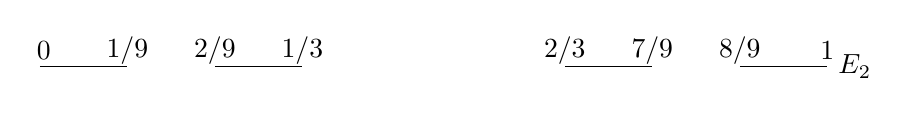
\begin{tikzpicture}[scale=10] % 调整图形的缩放比例
				\draw (0,0) -- (1/9,0);\draw (2/9,0) -- (1/3,0);\draw (6/9,0) -- (7/9,0);\draw (8/9,0) -- (1,0);
				\node(E21) at (0.005,0.02) {0};\node(E22) at (1/9,0.02) {1/9};
				\node(E23) at (2/9,0.02) {2/9};\node(E24) at (3/9,0.02) {1/3};
				\node(E25) at (6/9,0.02) {2/3};\node(E26) at (7/9,0.02) {7/9};
				\node(E27) at (8/9,0.02) {8/9};\node(E28) at (1,0.02) {1};
				\node(E2) at (1.035,0) {$E_2$};				
			\end{tikzpicture}
			\begin{tikzpicture}[scale=10] % 调整图形的缩放比例
				\draw (0,0) -- (1/27,0);\draw (2/27,0) -- (1/9,0);
				\draw (6/27,0) -- (7/27,0);\draw (8/27,0) -- (9/27,0);
				\draw (6/9,0) -- (19/27,0);\draw (20/27,0) -- (21/27,0);
				\draw (24/27,0) -- (25/27,0);\draw (26/27,0) -- (1,0);
				\node(E01) at (0.005,0.02) {0};
				\node(E02) at (1,0.02) {1};
				\node(E3) at (1.035,0) {$E_3$};				
			\end{tikzpicture}
			\begin{tikzpicture}[scale=10] % 调整图形的缩放比例		
				\draw (0,0) -- (1/81,0);\draw (2/81,0) -- (3/81,0);
				\draw (2/27,0) -- (7/81,0);\draw (8/81,0) -- (9/81,0);
				\draw (18/81,0) -- (19/81,0);\draw (20/81,0) -- (21/81,0);
				\draw (24/81,0) -- (25/81,0);\draw (26/81,0) -- (27/81,0);
				\draw (2/3,0) -- (55/81,0);\draw (56/81,0) -- (57/81,0);
				\draw (60/81,0) -- (61/81,0);\draw (62/81,0) -- (63/81,0);
				\draw (72/81,0) -- (73/81,0);\draw (74/81,0) -- (75/81,0);
				\draw (78/81,0) -- (79/81,0);\draw (80/81,0) -- (81/81,0);
				\node(E01) at (-0.005,0.02) {};
				\node(E02) at (1,0.02) {};
				\node(E4) at (1.035,0) {$E_4$};	
			\end{tikzpicture}
			\end{center} 
			\vspace{-1em}
			\caption{康托尔三分集}
			\label{Fi3}
		\end{figure}\vspace{-1em}
		
		由前面的定理可以知道,剩下的必是一个闭集,称它为康托尔三分集,记为$P$.
		这个闭集$P$具有哪些性质?
		
		\textbf{解:}
		
		(1)$P$\textbf{是完备集}\quad 由于$P$的邻接区间的做法,它们中的任何两个之间根本不存在公共端点,故$P$没有孤立点,因而$P$自密,又$P$是闭集,因此$P$是完备集.
		
		(2)$P$\textbf{没有内点}\quad 事实上,在$P$的作法中讲过,“去掉”过程进行到第$n$此为止时,剩下$2^n$个长度是$3^{-n}$的互相隔离的闭区间,因此任何一点$x_0\in P$必含在这$2^n$个闭区间的某一个里面.从而在$x_0$的任一领域$U(x_0,3^{-n})$内至少有一点不属于$P$,但$3^{-n}\to 0(n\to \infty)$,故$x_0$不可能是$P$的内点.
		
		$P$既然是没有内点的闭集,那么在任一开区间$I$内必至少含有开集$P^c$的一点,从而$I$内必至少有一子开区间,其中不含$P$的点.由疏朗集的定义,$P$是一个疏朗集合.
		
		(3)$[0,1]\setminus P$\textbf{是可数个互不相交的开区间,其长度之和为}1\quad 第$n$次去掉的$2^{n-1}$个长度为$3^{-n}$区间,因此$[0,1]\setminus P$中互不相交的开区间的长度之和为$$\sum_{n=1}^{\infty}\frac{2^{n-1}}{3^n}=1$$若$P$有“长度”,其“长度”只能为0.
		
		(4)$P$\textbf{的基数为$c$}\quad 若$[0,1]$中的数用三进制小数表示,第一次去掉的区间$\displaystyle \left(\frac{1}{3},\frac{2}{3}\right)$中每个数的第一位小数都是1,第二次去掉的两个区间中的每个数的第二位小数都是1.依此类推,第$n$次去掉的$2^{n-1}$个长度为$3^{-n}$区间中的每个数的第$n$位小数都是1,因此所有每位小数可以仅用0或2表示的数是永远不会去掉的.定义映射$\varphi :[0,1]\to P$,对$x\in [0,1]$,若$\displaystyle x=\sum_{n=1}^{\infty}\frac{a_n}{2^n}$(二进制小数表示),则$$\varphi (x)=\sum_{n=1}^{\infty}\frac{b_n}{3^n}\ \ \ (\text{三进制小数表示})$$其中$$b_n=\left\{\begin{aligned}
			&0,\ \ a_n=0\\&2,\ \ a_n=1
		\end{aligned}\right.$$由以上分析$\varphi(x)\in P$,且易知$\varphi$是单射.因此$|P|\ge |\varphi([0,1])|=|[0,1]|=c$.又$P\subset [0,1]$,又由$|P|\le |[0,1]|=c$,因此$|P|=c$.
		
		综上所述,我们将康托尔三分集的特点归纳为一句话:\uwave{\textbf{它是一个测度为零且基数为}} \uwave{$c$\textbf{的疏朗完备集}}.
	\end{liti}
	
	\section{测度论}
	
	\subsection{外测度}
	
	\begin{definition}
		设$E$为$\mathbb{R}^n$中任一点集,对于每一列覆盖$E$的开区间$\displaystyle \newcup{i=1}{\infty}I_i\supset E$,作出它的体积总和$\displaystyle \mu =\sum_{i=1}^{\infty}|I_i|$($\mu$可以等于$\infty$,不同的区间列一般有不同的$\mu$),所有这一切的$\mu$组成一个下方有界的数集,它的下确界(完全由$E$确定)称为$E$的\jiachu{勒贝格外测度},简称\textbf{L}\jiachu{外测度}或\jiachu{外测度},记为$m^*E$,即$$m^*E=\underset{E\subset \newcup{i=1}{\infty}I_i}{\inf}\sum_{i=1}^{\infty}|I_i|$$
	\end{definition}
	
	\begin{dinli}
		\setmainfont{Times New Roman}\kaishu
		
		(1)$m^*E\ge 0$,当$E$为空集时,$m^*E=0$;
		
		(2)设$A\subset B$,则$^*\le m^*$ (\jiachu{单调性});
		
		(3)$m^*\left(\newcup{i=1}{\infty}A_i\right)\le \displaystyle \sum_{i=1}^{\infty}m^*A_i$(\jiachu{次可数可加性}).
	\end{dinli}
	
	\subsection{可测集}
	
	\begin{dinli}
		设$E\subset \mathbb{R}^n$,则$m^*I=m^*(I\cap E)+m^*(I\cap E^c)$对$\mathbb{R}^n$中任何开区间都成立的充要条件是对$\mathbb{R}^n$中的任何点集$T$都有$$m^*T=m^*(T\cap E)+m^*(T\cap E^c)$$
	\end{dinli}
	
	\begin{definition}
		设$E$为$\mathbb{R}^n$中的点集,如果对任一点集$T$都有$$m^*T=m^*(T\cap E)+m^*(T\cap E^c)$$则称$E$是\textbf{L}\jiachu{可测的}.这时$E$的\textbf{L}\jiachu{外测度}$m^*E$即称为$E$的\textbf{L}\jiachu{测度},记为$mE$.L可测集全体记为$\mathscr{M}$.
	\end{definition}
	
	\begin{dinli}
		集合$E$可测的充要条件是对于任意$A\subset E,B\subset E^c$,总有$$m^*(A\cup B)=m^*A+m^*B$$
	\end{dinli}
	
	\begin{dinli}
		设$S_1,S_2$都可测,则$S_1\cup S_2$也可测,并且当$S_1\cap S_2=\varnothing$时,对于任意集合$T$总有$$m^*[T\cap (S_1\cup S_2)]=m^*(T\cap S_1)+m^*(T\cap S_2)$$
	\end{dinli}
	
	\begin{dinli}
		设$S_i(i=1,2,\cdots,n)$都可测,则$\newcap{i=1}{n}S_i$也可测.
	\end{dinli}
	
	\begin{dinli}
		设$S_1,S_2$都可测,则$S_1\setminus S_2$也可测.
	\end{dinli}
	
	\begin{dinli}
		设$\set{S_i}$是一列互不相交的可测集,则$\newcup{i=1}{\infty}S_i$也是可测集,且$$m\left(\bigcup_{i=1}^{\infty}S_i\right)=\sum_{i=1}^{\infty}mS_i$$
	\end{dinli}
	
	\begin{dinli}
		设$\set{S_i}$是一列可测集合,则$\newcup{i=1}{\infty}S_i$也是可测集合.
	\end{dinli}
	
	\begin{dinli}
		设$\set{S_i}$是一列可测集合,则$\newcap{i=1}{\infty}S_i$也是可测集合.
	\end{dinli}
	
	\begin{dinli}
		设$\set{S_i}$是一列递增的可测集合$$S_i\subset S_2\subset \cdots \subset S_n\subset \cdots$$令$\displaystyle S=\newcup{i=1}{\infty}S_i=\lim_{n\to \infty}S_n$,则$$mS=\lim_{n\to \infty}mS_n$$
	\end{dinli}
	
	\begin{dinli}
		设$\set{S_i}$是一列递减的可测集合$$S_i\supset S_2\supset \cdots \supset S_n\supset \cdots$$令$\displaystyle S=\newcap{i=1}{\infty}S_i=\lim_{n\to \infty}S_n$,则当$mS_1<\infty$时, $$mS=\lim_{n\to \infty}mS_n$$
	\end{dinli}
	
	\subsection{可测集类}
	
	\begin{dinli}
		\setmainfont{Times New Roman}\kaishu
		(1)凡外测度为零之集皆可测,称为零测度集;
		
		(2)零测度集之任何子集仍为零测度集;
		
		(3)有限个或可数个零测度集之和仍为零测度集.
	\end{dinli}
	
	\begin{dinli}
		凡开集、闭集皆可测.
	\end{dinli}
	
	\begin{definition}
		\setmainfont{Times New Roman}\kaishu
		设$\Omega$是由$\mathbb{R}^n$的一些子集类组成的集合类,如果$\Omega$满足条件
		
		(1)$\varnothing \in \Omega$;
		
		(2)若$E\in \Omega$,则$E^c\in \Omega$;
		
		(3)若$E_n\in \Omega,n=1,2,\cdots$,则$\newcup{n=1}{\infty}E_n\in \Omega$.
		
		则称$\Omega$是$\mathbb{R}^2$的一个$\bf{\sigma}$\jiachu{代数}.
	\end{definition}
	
	\begin{definition}
		\setmainfont{Times New Roman}\kaishu
		设$\Omega$是$\mathbb{R}^2$上的一个$\sigma$代数.如果定义在$\Omega$上的非负值集合函数$mu$满足条件
		
		(1)$\mu(\varnothing)=0$;
		
		(2)若$E_n\in \Omega,n=1,2,\cdots$,且任意$n\ne m$,$E_n\cap E_m\ne \varnothing$,有$$\mu\left(\bigcup_{n=1}^{\infty}E_n\right)=\sum_{n=1}^{\infty}\mu(E_n)$$则称$\mu$为$\Omega$上的\jiachu{(正)测度}.
	\end{definition}
	
	\begin{definition}
		设$\Sigma$是$\mathbb{R}^n$的一个子集族,则称所有包含$\Sigma$的$\sigma$代数的交集为$\Sigma$产生的$\sigma$代数.
	\end{definition}
	
	由于$\mathbb{R}^n$全体子集组成的子集类是包含$\Sigma$的$\sigma$代数,因此包含$\Sigma$的$\sigma$代数不是空集,并且是包含$\Sigma$的最小的$\sigma$代数.
	
	\begin{definition}
		\setmainfont{Times New Roman}\kaishu
		由$\mathbb{R}^n$中全体开集组成的子集类生成的$\sigma$代数,记为$\mathscr{B}_n$或$\mathscr{B}$,称为\jiachu{博雷尔(}\textit{Borel}\jiachu{)代数}.
	\end{definition}
	
	\begin{dinli}
		凡博雷尔集都是勒贝格可测集.
	\end{dinli}
	
	\begin{definition}
		若$\Omega$是$\mathbb{R}^n$上的一个$\sigma$代数,$\mu$是$\Omega$上的测度,则称$(\mathbb{R}^n,\Omega,\mu)$为\jiachu{测度空间}.
	\end{definition}
	
	\begin{definition}
		设集合$G$可表示为一列开集$\set{G_i}$之交集:$$G=\bigcap_{i=1}^{\infty}G_i$$则称$G$为$G_{\delta}$\jiachu{型集}.
		
		设集合$F$可表示为一列闭集$\set{F_i}$之交集:$$F=\bigcup_{i=1}^{\infty}F_i$$则称$F$为$F_{\sigma}$\jiachu{型集}.
	\end{definition}
	
	\begin{dinli}
		设$E$是任一可测集,则一定存在$G_{\delta}$型集$G$,使$G\supset E$,且$m(G\setminus E)=0$.
	\end{dinli}
	
	\begin{dinli}
		设$E$是任一可测集,则一定存在$F_{\sigma}$型集$F$,使$F\subset E$,且$m(E\setminus F)=0$.
	\end{dinli}
	
	\begin{liti}
		\setmainfont{Times New Roman}
		$E$是可测集的充要条件是:对任意的$\varepsilon>0$,存在开集$G_1,G_2,E\subset G_1,E^c\subset G_2,m(G_1\cap G_2)<\varepsilon$.
		
		\textbf{证明:}若$E$可测,则对任意$\varepsilon>0$,存在开集$E\subset G_1,E^c\subset G_2$,使得$$m(G_1\setminus E)<\frac{\varepsilon}{2},\ \ \ m(G_2\setminus E^c)<\frac{\varepsilon}{2}$$用集合运算的分配律得到$$\begin{aligned}
			G_1\cap G_2&=(E\cup (G_1\setminus E))\cap (E^c\cup (G_2\setminus E^c))\\&=((G_1\setminus E)\cap E^c)\cup (E\cap (G_2\setminus E^c))\cup ((G_1\setminus E)\cap (G_2\setminus E^c))\\&\subset (G_1\setminus E)\cup (G_2\setminus E^c)
		\end{aligned}$$因此$m(G_1\cap G_2)\le m(G_1\setminus E)+m(G_2\setminus E^c)<\varepsilon$.
		
		反之,由条件对任意$1/n>0$,存在开集$G_n,D_n$,满足条件$$E\subset G_n,E^c\subset D_n,\ \ m(G_n\cap D_n)<\frac{1}{n}$$令$F_n=D_n^c$,则$F_n$是闭集且$F_n\subset E\subset G_n$ $$G_n\setminus F_n=G_n\cap D_n,\ m(G_n\setminus F_n)=m(G_n\cap D_n)<\frac{1}{n}$$则$E$可测.
				
	\end{liti}
	
	
	\begin{dinli}
		\setmainfont{Times New Roman}\kaishu
		若$E$是一可测集,则
		
		(1)$mE=\inf\set{mG:G\text{是开集},E\subset G}$(\jiachu{外正规性});
		
		(2)$mE=\sup\set{mK:K\text{是紧集},K\subset E}$(\jiachu{内正规性}).
	\end{dinli}
	
	\begin{liti}
		\setmainfont{Times New Roman}
		设$A,B\subset \mathbb{R}^n$且$A\cup B$可测,$m(A\cup B)<\infty$.若$m(A\cup B)=m^*A+m^*B$,证明:$A$与$B$可测.
		
		\textbf{证明:}取$G_{\delta}$型集$G\supset A$,使得$mG=m^*A$,则$K=(A\cap B)\setminus G$可测,且$K\subset B$.因$A\cap B\subset ((A\cap B)\setminus G)\cap G$,则 $$m(A\cap B)\le m((A\cap B)\setminus G)+mG$$由此$$\begin{aligned}
		mK&=m((A\cap B)\setminus G)\ge m(A\cap B)-mG\\&=m^*A+m^*B-mG=m^*B
		\end{aligned}$$又$K\subset B$,有$mK\le m^*B$,于是$mK=m^*B$.用卡拉泰奥多里条件,得$$m^*B=m^*(B\cap K)+m^*(B\cap K^c)=mK+m^*(B\setminus K)$$因此$m^*(B\setminus K)=0$,从而$B\setminus K$可测.而$B+K\cup (B\setminus K)$也可测.同理$A$也可测.
	\end{liti}
	
	\subsection{不可测集}
	
	\begin{liti}
		\setmainfont{Times New Roman}
		\textbf{Vitali集}
		
		将$[0,1]$中的所有数依下法分类:两数$\xi,\eta$当且仅当$\xi -\eta$是有理数时,称$\xi$与$\eta$属于同一类,设$\xi\in [0,1]$中具有形式$\xi +r$($r$表示有理数)的点全体归为一类$E(\xi)$.这样,对于一个$\xi$有一类$E(\xi)$与之对应,且$\xi \in E(\xi)$,集$E(\xi)$不同于$E(\eta)$时,称$E(\xi)$与$E(\eta)$是不同的类,应当注意的是,当$\xi \ne \eta$时可能$E(\xi)=E(\eta)$.可以证明不同的两类$E(\xi)$和$E(\eta)$是不相交的:因为如果$E(\xi)\cap E(\eta)\ne \varnothing$,则必有$\zeta\in E(\xi)\cap E(\eta)$,因而$\zeta =\xi +r_{\xi},\zeta = \eta +r_{\eta}$,其中$r_{\xi} ,r_{\eta}$都是有理数.故得 $\eta=\xi+r_{\xi}-r_{\eta}$.现在假定$t\in E(\eta)$,则由$t=\eta +r=\xi+(r_{\xi}-r_{\eta}+r)$,得$t\in E(\xi)$.从而$E(\eta)\subset E(\xi)$.同理可得$E(\xi)\subset E(\eta)$,因此$E(\xi)=E(\eta)$.这与$E(\xi)$与$E(\eta)$是不同得两类之假设矛盾.
		
		这样一来,就把$[0,1]$区间分解成一族两两不交得集得并集.我们在每类集中去一个代表数,组成一个集$Z$(当$E(\xi)=E(\eta)$时,尽管$\xi$可以不等于$\eta$,但这是同一类,我们只取这类中得一个代表数).换句话说,对任何$\xi \in [0,1],E(\xi)\cap Z$时一个单元素集.
		
		接着我们把$[-1,1]$中的全体有理数排成一列$r_1,r_2,\cdots$,并记$Z_n=\tau_{r_n}Z=\set{x+r_n:x\in Z}$.我们证明这样作出的$Z_n$确实具有一种不可测集的性质.
		
		(1)对于任何$\xi\in[0,1],E(\xi)\cap Z$时单元素集,设为$\set{\eta},\eta\in Z$.因此$\xi -\eta$时有理数,由于$\xi,\eta$都在$[0,1]$中,所以$\xi -\eta \in[-1,1]$,因此$\xi -\eta $是$r_1,r_2,\cdots$中的某一个,设$\xi -\eta =r_{k'}$,可见$\xi\in \tau_{r_{k'}}Z=Z_{k'}$.这样我们就证明了任何$\xi \in[0,1]$必在$\newcup{n=1}{\infty}Z_n$中,即$[0,1]\subset \newcup{n=1}{\infty}Z_n$.
		
		(2)$Z_n$这里列集是两两不相交的,因为如果存在两个不同的正整数$l$及$n$,使$\xi\in Z_l\cap Z_n$,那么$\xi -r_l,\xi -r_n$都属于$Z$.但这两个数属于同一类,且因$l\ne n$,必定$r_l\ne r_n$.所以$\xi-r_l$与$\xi-r_n$是不同的数,但由$Z$的作法,它与每个类的交集只有一个元,这就产生了矛盾.由此证明了$\set{Z_n}$这一列集使互不相交的.另外由$Z\subset [0,1],r_n\in [-1,1]$,即知$Z_n\subset [-1,2]$,所以$\newcup{n=1}{\infty}Z_n\subset [-1,2]$.
		
		由一种不可测集的性质:
		
		(1)$\newcup{n=1}{\infty}Z_n$包含一个区间(例如$\newcup{n=1}{\infty}Z_n\supset[0,1]$);
		
		(2)$\set{Z_n}$是一列互不相交的集,而且$\newcup{n=1}{\infty}Z_n$是有界集(例如$\newcup{n=1}{\infty}Z_n\subset[-1,2]$).
		
		确定$Z$是不可测集.
	\end{liti}
	
	\section{可测函数}
	
	\subsection{可测函数及其性质}
	
	\begin{definition}
		设$f(x)$是定义再可测集$E\subset \mathbb{R}^n$的实函数.如果对于任何有限实数$a$,$E[f>a]$都是可测集,则称$f(x)$为定义在$E$上的\jiachu{可测函数}.
	\end{definition}
	
	\begin{dinli}
		\setmainfont{Times New Roman}\kaishu
		设$f(x)$实定义再可测集$E$上的实函数,下列任一条件都是$f(x)$在$E$上可测的充要条件:
		
		(1)对任何有限实数$a$,$E[f\ge a]$都可测;
		
		(2)对任何有限实数$a$,$E[f< a]$都可测;
		
		(3)对任何有限实数$a$,$E[f\le a]$都可测;
		
		(4)对任何有限实数$a,b(a<b)$,$E[a\le f<b]$都可测(但充分性要假定$f(x)$实有限函数).
	\end{dinli}
	
	\begin{dinli}
		设$f(x)$在$E$上可测,则$E[f=a]$总可测,不论$a$实有限实数或$\pm \infty$.
	\end{dinli}
	
	\begin{definition}
		定义在$E\subset \mathbb{R}^n$上的实函数$f(x)$称为在$x_0\in E$\jiachu{连续},如果$y_0=f(x_0)$有限,而且对于$y_0$的任一领域$V$,存在$x_0$的某领域$U$,使得$f(U\cap E)\subset V$,即只要$x\in E$且$x\in U$时,便有$f(x)\in V$.如果$f(x)$在$E$中每一点都连续,则称$f(x)$\jiachu{在}$E$\jiachu{上连续}.
	\end{definition}
	
	\begin{dinli}
		可测集$E\subset \mathbb{R}^n$上的连续函数是可测函数.
	\end{dinli}
	
	\begin{dinli}
		\setmainfont{Times New Roman}\kaishu
		(1)设$f(x)$是可测集$E$上的可测函数,而$E_1\subset E$为$E$的可测子集,则$f(x)$看作定义在$E_1$上的函数时,它是$E_1$上的可测函数.
		
		(2)设$f(x)$定义在有限个可测集$E_i(i=1,2,\cdots,s)$的并集$E=\newcup{i=1}{s}E_i$上,且$f(x)$在每个$E_i$上都可测,则$f(x)$在$E$上也可测.
	\end{dinli}
	
	\begin{definition}
		设$f(x)$的定义域$E$可分为有限个互不相交的可测集$E_1,E_2,\cdots,E_s,E=\newcup{i=1}{s}E_i$,使$f(x)$在每个$E_i$上都等于某常数$c_i$,则称$f(x)$为\jiachu{简单函数}.
	\end{definition}
	
	\begin{liti}
		\setmainfont{Times New Roman}
		设$f(x)$与$g(x)$为$E$上的可测函数,证明:$E[f>g]$与$E[f\ge g]$都是可测集.
		
		\textbf{证明:}因$E[f\ge g]=E\setminus E[f<g]$,故只需证明$E[f>g]$可测.设$x_0\in E[f>g]$,亦即$f(x_0)>g(x_0)$,则必存在有理数$r$,使$f(x_0)>r>g(x_0)$,亦即$$x_0\in E[f>r]\cap E[g<r]$$反之亦然.
		
		因此,设有理数全体为$r_1,r_2,\cdots$,则$$E[f>g]=\bigcup_{n=1}^{\infty}(E[f>r_n]\cap E[g<r_n])$$
		等式的右边显然是可测集.
	\end{liti}
	
	\begin{dinli}
		\setmainfont{Times New Roman}\kaishu
		设$f(x),g(x)$在$E$上可测,则下列函数(假定它们在$E$上有意义)皆在$E$上可测:
		
		(1)$f(x)+g(x)$;		
		(2)$|f(x)|$;		
		(3)$\displaystyle \frac{1}{f(x)}$;		
		(4)$f(x)\cdot g(x)$.
	\end{dinli}
	
	\begin{dinli}
		设$\{f_n(x)\}$是$E$上一列(或有限个)可测函数,则$\displaystyle \mu(x)=\inf_nf_n(x)$与$\displaystyle \lambda(x)=\sup_nf_n(x)$都在$E$上可测.
	\end{dinli}
	
	\begin{dinli}
		设$\{f_n(x)\}$是$E$上一列可测函数,则$\displaystyle F(x)=\liminf_{n\to \infty} f_n(x),G(x)=\limsup_{n\to \infty} f_n(x)$也在$E$上可测,特别当$\displaystyle F(x)=\lim_n f_n(x)$存在时,它也在$E$上可测.
	\end{dinli}
	
	\begin{dinli}
		\setmainfont{Times New Roman}
		\textbf{(可测函数与简单函数的关系)}\ \kaishu
		
		(1)若$f(x)$在$E$上非负可测,则存在可测简单函数列$\{\varphi _k(x)\}$,使得对任意$x\in E$,$\varphi _k(x)\le \varphi _{k+1}(x)(k= 1,2,\cdots)$,且$\displaystyle \lim_{k\to \infty}\varphi_k(x)=f(x)$;
		
		(2)若$f(x)$在$E$上可测,则存在可测简单函数列$\{\varphi _k(x)\}$,使得对任意$x\in E$,$\displaystyle \lim_{k\to \infty}\varphi_k(x)=f(x)$.若$f(x)$还在$E$上有界,则上述收敛可以是一致的.
	\end{dinli}
	
	\begin{definition}
		设$\pi$是一个与集合$E$的点$x$有关的命题,如果存在$E$的子集$M$,满足$mM=0$,使得$\pi$在$E\setminus M$上恒成立,也就是说,$E\setminus E[\pi \text{成立}]$是零测度集,则我们称$\pi$在$E$上\jiachu{几乎处处}成立,或说$\pi\  \aevery$于$E$.
	\end{definition}
	
	\begin{dinli}
		\setmainfont{Times New Roman}
		\textbf{(叶戈罗夫定理)}\ \kaishu 设$mE<\infty$,$\{f_n\}$是$E$上一列$\aevery$收敛于一个$\aevery$有限的函数$f$的可测函数,则对任意$\delta >0$,存在子集$E_{\delta}\subset E$,使$\set{f_{n}}$在$E_{\delta}$上一致收敛,且$m(E\setminus E_{\delta})<\delta$.		
	\end{dinli}
	
	\subsection{可测函数的构造}
	
	\begin{dinli}
		\setmainfont{Times New Roman}
		\textbf{(卢津定理)}\ \kaishu 设$f(x)$是$E$上$\aevery$有限的可测函数,则对任意$\delta >0$,存在闭子集$F_{\delta}\subset E$,使$f(x)$在$F_{\delta}$上是连续函数,且$m(E\setminus F_{\delta})<\delta $.
	\end{dinli}
	\setmainfont{Times New Roman}
	
	\uwave{简而言之,在$E$上$\aevery$有限的可测函数是“基本上连续”的函数.}
	
	\begin{dinli}
		设$f(x)$是$E\subset \mathbb{R}$上$\aevery$有限的可测函数,则对任意$\delta >0$,存在闭集$F\subset E$及整个$\mathbb{R}$上的连续函数$g(x)$($F$及$g(x)$依赖于$\delta$),使得在$F$上$g(x)=f(x)$,且$m(E\setminus F)<\delta$.此外还可要求$$\sup_{\mathbb{R}}g(x)=\sup_F f(x)\ \ \ \ \ \ \ \inf_{\mathbb{R}}g(x)=\inf_F f(x)$$
	\end{dinli}
	
	\subsection{依测度收敛}
	
	\begin{definition}
		设$f_n$是$E\subset \mathbb{R}^q$上一列$\aevery$有限的可测函数,若有$E$上$\aevery$有限的可测函数$f(x)$满足对任意$\sigma>0$,有$\displaystyle \lim_n mE[|f_n-f|\ge \sigma]=0$,则称函数列$\set{f_n}$\jiachu{依测度收敛于}$f$,或\jiachu{度量收敛}于$f$,记为$f_n(x)\Rightarrow f(x)$.
	\end{definition}
	
	\begin{liti}
		\setmainfont{Times New Roman}
		依测度收敛而处处不收敛的函数列.
		
		取$E=(0,1]$,将$E$等分,定义两个函数:$$f_1^{(1)}(x)=\left\{\begin{aligned}
			&1&x\in \left(0,\frac{1}{2}\right]\\&0&x\in \left(\frac{1}{2},1\right]
		\end{aligned}\right.$$  $$f_2^{(1)}(x)=\left\{\begin{aligned}
		&0&x\in \left(0,\frac{1}{2}\right]\\&1&x\in \left(\frac{1}{2},1\right]
		\end{aligned}\right.$$然后将$(0,1]$四等分、八等分,等等.一般地,对每个$n$,作$2^n$个函数:$$f_j^{(n)}(x)=\left\{\begin{aligned}
		&1&x\in \left(\frac{j-1}{2^n},\frac{j}{2^n}\right]\\&0&x\notin \left(\frac{j-1}{2^n},\frac{j}{2^n}\right]
		\end{aligned}\right.\ \ \ j=1,2,\cdots,2^n$$
		
		我们吧$\set{f_j^{(n)}:j=1,2,\cdots,2^n}$先按$n$后按$j$的顺序逐个地排成一列:$$f_1^{(1)}(x),f_2^{(1)}(x),\cdots,f_1^{(n)}(x),f_2^{(n)}(x),\cdots,f_{2^n}^{(n)}(x),\cdots$$ $f_j^{(n)}(x)$在这个序列中是第$N=2n-2+j$个函数.可以证明这个序列是依测度收敛于零的.这是因为对任何$\sigma>0,E[|f_j^{(n)}-0|\ge \sigma]$或是空集(当$\sigma >1$),或是$\displaystyle \left(\frac{j-1}{2^n},\frac{j}{2^n}\right]$(当$0<\sigma \le 1$),所以$$m(E[|f_j^{(n)}-0|\ge \sigma ])\le \frac{1}{2^n}\ \ \ \text{(当$\sigma >1$时,左端为$0$)}$$由于当$N=2^n-2+j(j=1,2,\cdots,2^n)$趋于$\infty$时,$n\to \infty$.由此可见$$\lim_{N\to\infty}m(E[|f_j^{(n)}-0|\ge \sigma ])=0$$即$f_j^{(n)}(x)\Rightarrow 0$.
		
		但是函数列在$(0,1]$上的任何一点都不收敛.事实上,对任何点$x_0\in (0,1]$,无论$n$多么大,总存在$j$,使$\displaystyle x_0\in \left(\frac{j-1}{2^n},\frac{j}{2^n}\right]$,因而$f_j^{(n)}(x_0)=1$,然而$f_{n+1}^{(n)}(x_0)=0$或$f_{j-1}^{(n)}(x_0)=0$换而言之,对任何$x_0\in(0,1]$,在$\{f_j^{(n)}(x_0)\}$中必有两个子列,一个恒为$1$,另一个恒为$0$,所以序列在$(0,1]$上任何点都是发散的.
	\end{liti}
	
	\begin{liti}
		\setmainfont{Times New Roman}
		取$E=(0,\infty)$,作函数列$$f_n(x)=\left\{\begin{aligned}
			&1&x\in (0,n]\\&0&x\in(n,\infty)
		\end{aligned}\right.\ \ \ n=1,2,\cdots$$显然$f_n(x)\to 1(n\to \infty)$,当$x\in E$.但是当$0<\sigma <1$时,$$E[|f_n-1|\ge \sigma]=(0,\infty)$$且$m(n,\infty)=\infty$.这说明$\{f_n\}$不依测度收敛于$1$.
	\end{liti}
	
	\begin{dinli}
		\setmainfont{Times New Roman}
		\textbf{(里斯定理)}\ \kaishu 设在$E$上$\{f_n\}$依测度收敛于$f$,则存在子列$\{f_{n_i}\}$在$E$上$\aevery$收敛于$f$.
	\end{dinli}
	
	\begin{dinli}
		\setmainfont{Times New Roman}
		\textbf{(勒贝格)}\ \kaishu 设
		
		(1)$mE<\infty$;
		
		(2)$\{f_n\}$是$E$上$\aevery$有限的可测函数列;
		
		(3)$\{f_n\}$在$E$山$\aevery$收敛于$\aevery$有限的函数$f$,
		
		\hspace{-2em}则$$f_n(x)\Rightarrow f(x)$$
	\end{dinli}
	
	\begin{dinli}
		设$f_n(x)\Rightarrow f(x),f_n(x)\Rightarrow g(x)$,则$f(x)=g(x)$在$E$上几乎处处成立.
	\end{dinli}
	
	\begin{liti}
		\setmainfont{Times New Roman}
		设$E\subset \mathbb{R}$,$f(x)$是$E$上$\aevery$有限的可测函数.证明:存在定义在$\mathbb{R}$上的一列连续函数$\{g_n(x)\}$,使得$$\lim_{n\to \infty}g_n(x)=f(x)\ \aevery \text{于}E$$
		
		\textbf{证明:}由于涉及可测函数与连续函数之间的关系,我们首先会想到应用卢津定理.因为$f(x)$在$E$上可测,由卢津定理,对任何正整数$n$,存在$E$的可测子集$E_n$,使得$\displaystyle m(E\setminus E_n)<\frac{1}{2}$,同时存在定义在$\mathbb{R}$上的连续函数$g_n(x)$,使得当$x\in E_n$时有$g_n(x)=f(x)$.所以对任意的$\eta>0$,有$$E[|f-g_n|\ge \eta]\subset E\setminus E_n$$由此可得$$mE[|f-g_n|\ge \eta]\le  m(E\setminus E_n)<\frac{1}{n}$$因此$$\lim_{n\to \infty}mE[|f-g_n|\ge \eta]=0$$即$g_n(x)\Rightarrow f(x)$,由里斯定理。存在$\{g_n\}$的子列$\{g_{n_k}\}$,使得$$\lim_{k\to \infty}g_{n_k}(x)=f(x)\ \aevery \text{于}E$$
		
	\end{liti}
	
	\section{积分论}
	
	\subsection{黎曼积分}
	
	\subsubsection{$R$可积的必要条件}
	
	\begin{dinli}
		\setmainfont{Times New Roman}
		\kaishu
		若函数$f$在$[a,b]$上可积,则$f$在$[a,b]$上必定有界.
	\end{dinli}
	
	\subsubsection{$R$可积的充要条件}
	
	\begin{dinli}
		\setmainfont{Times New Roman}
		\textbf{(可积的第一充要条件)}\ \kaishu
		函数$f$在$[a,b]$上可积的充要条件是:$f$在$[a,b]$上的上积分与下积分相等,即$$S=s$$
	\end{dinli}
	
	\begin{dinli}
		\setmainfont{Times New Roman}
		\textbf{(可积的第二充要条件)}\ \kaishu
		函数$f$在$[a,b]$上可积的充要条件是:任给$\varepsilon >0$,总存在某一分割$T$,使得$$S(T)-s(T)<\varepsilon ,\text{即}\sum_{i=1}^{n}\omega_i \Delta x_i<\varepsilon$$其中$\omega_i=M_i-m_i$($f$在$\Delta_i$上的振幅),$i=1,2,\cdots,n$.
	\end{dinli}
	
	\begin{dinli}
		\setmainfont{Times New Roman}
		\textbf{(可积的第三充要条件)}\ \kaishu
		函数$f$在$[a,b]$上可积的充要条件是:任给正数$\varepsilon,\eta$,总存在某一分割$T$,使得属于$T$的所有小区间中,对应于振幅$\omega_{k'}\ge \varepsilon$的那些小区间$\Delta_{k'}$的总长$\displaystyle \sum_{k'}\Delta x_{k'}<\eta$.
	\end{dinli}
	
	\subsubsection{$R$积分的局限性}
	
	(1)\textbf{$R$积分与极限可交换的条件太苛刻}
	
	我们知道一列$R$积分函数的极限函数(即使有界)不一定$R$可积.因此在积分与极限交换问题上,$R$积分的局限性就特别突出,大家知道:为了使$$\reint{a}{b}{\lim_{n\to \infty}f_n(x)}x=\lim_{n\to \infty}\reint{a}{b}{f_n(x)}x$$对一列收敛的$R$可积函数$\set{f_n}$能成立,通常需要对$\set{f_n}$加上一致收敛的条件.可是这一充分条件不但非常苛刻而且检验起来也非常不方便,因而大大降低了$R$积分的效果.
	
	(2)\textbf{$R$积分运算不完全使微分运算的逆运算}
	
	我们知道任一$R$可积函数$f(x)$的变动上限积分$\displaystyle F(x)=\reint{a}{x}{f(t)}x$在$f(x)$的所有连续点都有$F'(x)=f(x)$,换言之,就是积分后再微分可以还原($f(x)$的不连续点构成零集,可忽略不计).
	
	但是另一方面有例子说明,一个可微函数$F(x)$的导函数$f(x)$即使有界也不一定$R$可积[沃尔泰拉(Volterra)的例],因此也就无法成立牛顿-莱布尼茨(Newton-Leibniz)公式$$F(x)-F(a)=\reint{a}{x}{f(x)}x$$所以在$R$积分范围内,积分运算只是部分地称为微分运算之逆.
	
	
	\subsection{非负可测函数的勒贝格积分}
	
	\subsubsection{简单函数}
	
	\begin{definition}
		设$E\subset \mathbb{R}^n$为可测集,$\varphi(x)$为$E$上的一个非负简单函数,即$E$表示为有限个互不相交的可测集$E-1,E_2,\cdots,E_k$之并,而在每个$E_i$上$\varphi(x)$取非负常数值$c_i$,也就是说$$\varphi(x)=\sum_{i=1}^{k}c_i\chi_{E_i}(x)$$这里$\chi_{E_i}(x)$是$E_i$的特征函数.
		
		$\varphi(x)$在$E$上的勒贝格积分,定义为$$\reint{E}{}{\varphi(x)}x=\sum_{i=1}^{k}c_imE_i$$
		
		设$A\subset E$为可测子集,$\varphi(x)$在$A$上的勒贝格积分定义为$\varphi$在$A$上的限制$\varphi |_A$在$A$上的勒贝格积分,于是$$\reint{A}{}{\varphi(x)}x=\sum_{i=1}^{k}c_im(A\cap E_i)$$
	\end{definition}
	
	\begin{dinli}
		\setmainfont{Times New Roman}\kaishu
		设$E\subset \mathbb{R}^n$为可测集,$\varphi(x)$为$E$上的一个非负简单函数.我们有
		
		(1)对于任意的非负实数$c$,有$$\reint{E}{}{c\varphi(x)}x=c\reint{E}{}{\varphi(x)}x$$
		
		(2)设$A$和$B$是$E$的两个互不相交的可测子集,则$$\reint{A\cup B}{}{\varphi(x)}x=\reint{A}{}{\varphi(x)}x+\reint{B}{}{\varphi(x)}x$$
		
		(3)设$\set{A_n}_{n=1}^{\infty}$是$E$的一列可测子集,满足$A_1\subset A_2\subset \cdots\subset A_n\subset A_{n+1}\subset \cdots$及$\newcup{n=1}{\infty}A_n=E$,则$$\lim_{n\to \infty}\reint{A_n}{}{\varphi(x)}x=\reint{E}{}{\varphi(x)}x$$
	\end{dinli}
	
	\begin{dinli}
		\setmainfont{Times New Roman}\kaishu
		设$E\subset \mathbb{R}^n$为可测集,$\varphi(x)$和$\psi(x)$都是$E$上的非负简单函数,则
		
		(1)$\reint{E}{}{\varphi(x)}x+\reint{E}{}{\psi(x)}x=\reint{E}{}{(\varphi(x)+\psi(x))}x$;
		
		(2)对于任意的非负实数$\alpha$和$\beta$,有$$\alpha \reint{E}{}{\varphi(x)}x+\beta \reint{E}{}{\psi(x)}x=\reint{E}{}{(\alpha \varphi(x)+\beta \psi(x))}x$$
	\end{dinli}
	
	\subsubsection{可测函数}
	
	\begin{definition}
		设$E\subset \mathbb{R}^n$为可测集,$f(x)$是$E$上的一个非负可测函数,$f(x)$在$E$上的\jiachu{勒贝格积分}定义为$$\reint{E}{}{f(x)}x=\sup\left\{\reint{E}{}{\varphi(x)}x:\varphi(x)\text{是$E$上的简单函数,且$x\in E$时,}0\le \varphi(x)\le f(x)\right\}$$ 显然$0\le \reint{E}{}{f(x)}x\le \infty$,若$\reint{E}{}{f(x)}x<\infty$,则称$f(x)$在$E$上\jiachu{勒贝格可积}.
		
		设$A\subset E$为可测集,则$f(x)$在$A$上的勒贝格积分定义为$f$在$A$上的限制$f|_A$在$A$上的勒贝格积分.我们有$$\reint{A}{}{f(x)}x=\reint{E}{}{f(x)\chi_A(x)}x$$
	\end{definition}
	
	\begin{dinli}
		\setmainfont{Times New Roman}\kaishu
		设$E\subset \mathbb{R}^n$为可测集,$F(x)$为$E$上的一个非负可测函数,我们有
		
		(1)若$mE=0$,则$\reint{E}{}{f(x)}x=0$;
		
		(2)若$\reint{E}{}{f(x)}x=0$,则$f(x)=0\ \aevery $于$E$;
		
		(3)若$\reint{E}{}{f(x)}x<\infty$,则$0\le f(x)<\infty\ \aevery$于$E$;
		
		(4)设$A$和$B$为$E$的两个互不相交的可测子集,则$$\reint{A\cup B}{}{f(x)}x=\reint{A}{}{f(x)}x+\reint{B}{}{f(x)}x$$
	\end{dinli}
		
	\begin{dinli}
		\setmainfont{Times New Roman}\kaishu
		设$E\subset \mathbb{R}^n$为可测集,$f(x)$和$g(x)$都是$E$上的非负可测函数.我们有
		
		(1)若$f(x)\le g(x)\ \aevery$于$E$,则$\reint{E}{}{f(x)}x\le \reint{E}{}{f(x)}x$;这时,若$g(x)$在$E$上$L$可测,则$f(x)$也在$E$上$L$可测;
		
		(2)若$f(x)=g(x)\ \aevery$于$E$,则$\reint{E}{}{f(x)}x=\reint{E}{}{g(x)}x$;特别地,若$f(x)=0\ \aevery$于$E$,则$\reint{E}{}{f(x)}x=0$.
	\end{dinli}
	
	\begin{dinli}
		\setmainfont{Times New Roman}\textbf{(莱维(Levi)定理)} \ \ \ \kaishu
		设$E\subset \mathbb{R}^n$为可测集,$\set{f_n}_{n=1}^{\infty}$为$E$上的一列非负可测函数,当$x\in E$时对于任一正整数$n$,有$f_n(x)\le f_{n+1}(x)$,令$\displaystyle f(x)=\lim_{n\to \infty}f_n{(x)},x\in E$,则$$\lim_{n\to \infty}\reint{E}{}{f_n(x)}x=\reint{E}{}{f(x)}x$$
	\end{dinli}
	
	\begin{dinli}
		设$E\subset \mathbb{R}^n$为可测集,$f(x)$和$g(x)$都是$E$上的非负可测函数,$\alpha$和$\beta $都是非负实数,则$$\reint{E}{}{(\alpha f(x)+\beta g(x))}x=\alpha \reint{E}{}{f(x)}x+\beta \reint{E}{}{g(x)}x$$特别地$$\reint{E}{}{\alpha f(x)}x=\alpha \reint{E}{}{f(x)}x$$  $$\reint{E}{}{(f(x)+g(x))}x=\reint{E}{}{f(x)}x+\reint{E}{}{g(x)}x$$
	\end{dinli}
	
	\begin{dinli}
		\setmainfont{Times New Roman}\textbf{(逐项积分定理)}\kaishu\ \ \ 
		设$E\subset \mathbb{R}^n$为可测集,$\set{f_n}_{n=1}^{\infty}$为$E$上的一列非负可测函数,则$$\reint{E}{}{\left(\sum_{n=1}^{\infty}f_n(x)\right)}x=\sum_{n=1}^{\infty}\reint{E}{}{f_n(x)}x$$
	\end{dinli}
	
	\begin{dinli}
		\setmainfont{Times New Roman}\textbf{(法图(Fatou)引理)}\kaishu\ \ \ 
		设$E\subset \mathbb{R}^n$为可测集,$\set{f_n}_{n=1}^{\infty}$为$E$上的一列非负可测函数,则$$\reint{E}{}{\liminf_{n\to \infty}f_n(x)}x\le \liminf_{n\to \infty}\reint{E}{}{f_n(x)}x$$
	\end{dinli}
	
	\subsection{一般可测函数的勒贝格积分}
	
	\begin{definition}
		设$E\subset \mathbb{R}^n$为可测集,$f(x)$为$E$上的可测函数.令$$f^+(x)=\max\{f(x),0\},\ \ \ f^-(x)=\max\set{-f(x),0}$$则$f^+$和$f^-$都是$E$上的非负可测函数,当$x\in E$时,$$f^+(x)-f^-(x)=f(x),\ \ \ f^+(x)+f^-(x)=|f(x)|$$
		
		若$\reint{E}{}{f^+(x)}x$和$\reint{E}{}{f^-(x)}x$中至少一个有限,则称$f$在$E$上积分确定,称$\reint{E}{}{f^+(x)}x-\reint{E}{}{f^-(x)}x$为$f$在$E$上的\jiachu{勒贝格积分},记作$\reint{E}{}{f(x)}x$.
		
		若$\reint{E}{}{f^+(x)}x$和$\reint{E}{}{f^-(x)}x$都有限,则称$f$在$E$上\jiachu{勒贝格可积},简称\jiachu{$L$可积}.
	\end{definition}
	
	\begin{dinli}
		\setmainfont{Times New Roman}\kaishu
		设$E\subset \mathbb{R}^n$为可测集,我们有
		
		(1)若$E\ne \varnothing$但$mE=0$,则$E$上任何实函数$f$都在$E$上$L$可积,且$\reint{E}{}{f(x)}x=0$;
		
		(2)若$f\in L(E)$,则$mE[|f|=\infty]=0$,即$|f(x)|<\infty \ \aevery$于$E$;
		
		(3)设$f$在$E$上积分确定,则$f$在$E$的任一可测子集$A$上也积分确定,又若$E=A\cup B$,这里$A$和$B$都是$E$的可测子集,且$A\cap B=\varnothing$,则$$\reint{E}{}{f(x)}x=\reint{A}{}{f(x)}x+\reint{B}{}{f(x)}x$$
		
		(4)设$f$在$E$上积分确定且$f(x)=g(x)\ \aevery$于$E$,则$g$也在$E$上积分确定,且$$\reint{E}{}{f(x)}x=\reint{E}{}{g(x)}x$$
		
		(5)设$f$和$g$都在$E$上积分确定,且$f(x)\le g(x)\ \aevery$于$E$,则$$\reint{E}{}{f(x)}x\le \reint{E}{}{g(x)}x$$特别地,若$mE<\infty$且$b\le f(x)\le B\ \aevery$于$E$,则$$bmE\le \reint{E}{}{f(x)}x\le BmE$$
		
		(6)设$f$在$E$上$L$可积,则$|f|$也在$E$上$L$可积,且$$\left|\reint{E}{}{f(x)}x\right|\le \reint{E}{}{|f(x)|}x$$
		
		(7)设$f$是$E$上的可测函数,$g$是$E$上的非负$L$可积函数,且$|f(x)|\le g(x)\ \aevery$于$E$,则$f$也在$E$上$L$可积且$$\left|\reint{E}{}{f(x)}x\right|\le \reint{E}{}{|f(x)|}x\le \reint{E}{}{g(x)}x$$
	\end{dinli}
	
	\begin{dinli}
		\setmainfont{Times New Roman}\kaishu
		设$E\subset \mathbb{R}^n$为可测集,$f$和$g$都是$E$上的$L$可积函数,则
		
		(1)对于任意的$\lambda \in \mathbb{R}$,$\lambda f$在$E$上$L$可积,且$$\reint{E}{}{\lambda f(x)}x=\lambda \reint{E}{}{f(x)}x$$
		
		(2)$f+g$在$E$上$L$可积,且$$\reint{E}{}{(f(x)+g(x))}x=\reint{E}{}{f(x)}x+\reint{E}{}{g(x)}x$$
		
		(3)对于任意的$\alpha ,\beta \in \mathbb{R}$,$\alpha f+\beta g$在$E$上$L$可积,且$$\reint{E}{}{(\alpha f(x)+\beta g(x))}x=\alpha\reint{E}{}{f(x)}x+\beta \reint{E}{}{g(x)}x$$
	\end{dinli}
	
	\begin{dinli}
		\setmainfont{Times New Roman}\textbf{(积分的绝对连续性)}\kaishu\ \ \ 
		设$E\subset \mathbb{R}^n$为可测集,$f\in L(E)$,则对于任意的$\varepsilon>0$,存在$\delta>0$,使得对于任意的可测集$A\subset E$,只要$mA<\delta$,就有$$\left|\reint{E}{}{f(x)}x\right|\le \reint{A}{}{|f(x)|}x<\varepsilon$$
	\end{dinli}
	
	\begin{dinli}
		\setmainfont{Times New Roman}\textbf{(积分的可数可加性)}\kaishu\ \ \ 
		设$E\subset \mathbb{R}^n$为可测集,$E=\newcup{n=1}{\infty}E_n$,这里每个$E_n$都是可测集,且$i\ne j$时,$E_i\cap E_j=\varnothing$,设$f$在$E$上积分确定,则$$\reint{E}{}{f(x)}x=\sum_{n=1}^{\infty}\reint{E_n}{}{f(x)}x$$
	\end{dinli}
	
	\begin{dinli}
		\setmainfont{Times New Roman}\textbf{(勒贝格控制收敛定理)}\kaishu\ \ \ 
		设$E\subset \mathbb{R}^n$为可测集,$\set{f_n}_{n=1}^{\infty}$为$E$上的一列可测函数.$F$是$E$上的非负$L$可积函数,如果对于任意的正整数$n$,$|f_n(x)|\le F(x)\ \aevery$于$E$,且$\displaystyle \lim_{n\to \infty}f_n(x)=f(x)\ \aevery$于$E$,则
		
		(1)$\displaystyle \lim_{n\to \infty}\reint{E}{}{|f_n(x)-f(x)|}x=0$;\vspace{0.5em}
		
		(2)$\displaystyle \lim_{n\to \infty}\reint{E}{}{f_n(x)}x=\reint{E}{}{f(x)}x$.
	\end{dinli}
	
	\begin{dinli}
		\setmainfont{Times New Roman}\kaishu
		设$E\subset \mathbb{R}^n$为可测集,$f$和$f_n(n=1,2,3,\cdots)$都是$E$上的可测函数,$F$是$E$上的非负$L$可积函数,如果$|f_n(x)|\le F(x) \ \aevery$于$E$,且$n\to \infty$时$f_n\Rightarrow f$,则
		
		(1)$\displaystyle \lim_{n\to \infty}\reint{E}{}{|f_n(x)-f(x)|}x=0$;\vspace{0.5em}
		
		(2)$\displaystyle \lim_{n\to \infty}\reint{E}{}{f_n(x)}x=\reint{E}{}{f(x)}x$.
	\end{dinli}
	
	\begin{dinli}
		设$E\subset \mathbb{R}^n$为可测集,$\set{f_n}_{n=1}^{\infty}$为$E$上的一列$L$可积函数.如果正项级数$\displaystyle \sum_{n=1}^{\infty}\reint{E}{}{|f_n(x)|}x$收敛,则函数项级数$\displaystyle \sum_{n=1}^{\infty}f_n(x)$在$E$上$\aevery$收敛,其和函数在$E$上$L$可积,且$$\reint{E}{}{\left(\sum_{n=1}^{\infty}f_n(x)\right)}x=\sum_{n=1}^{\infty}\reint{E}{}{f_n(x)}x$$
	\end{dinli}
	
	\begin{dinli}
		设$E\subset \mathbb{R}^n$为可测集,$f(x,t)$是$E\times (a,b)$上的实函数.如果对于任意的$t\in (a,b)$,$f(x,t)$作为$x$的函数在$E$上$L$可积,对于$\aevery$的$x\in E$,$f(x,t)$作为$t$的函数在$(a,b)$上可导且$\left|\displaystyle \frac{\partial}{\partial t}f(x,t)\right|\le F(x)$,这里$F$是$E$上某个非负$L$可积函数,则$\reint{E}{}{f(x,t)}x$作为$t$的函数在$(a,b)$上可导,且$$\frac{\mathrm{d}}{\mathrm{d}t}\reint{E}{}{f(x,t)}x=\reint{E}{}{\frac{\partial }{\partial t}f(x,t)}x$$
	\end{dinli}
	
	\begin{liti}
		\setmainfont{Times New Roman}
		设$f\in L[a,b]$,则对于任意的$\varepsilon >0$,存在$g\in C[a,b]$,使得$$\reint{[a,b]}{}{|f(x)-g(x)|}x< \varepsilon$$
		
		\textbf{证明:}由于$f\in L[a,b]$,故$f^+$和$f^-$都在$[a,b]$上非负$L$可积.对于任意的$\varepsilon>0$,由勒贝格积分的定义可得,存在$[a,b]$上的两个非负简单函数$\varphi_1$和$\varphi_2$,使得$x\in [a,b]$时,$0\le \varphi_1(x)\le f^+(x)$,$0\le \varphi_2(x)\le f^-(x)$.且$$\reint{[a,b]}{}{f^+(x)}x-\frac{\varepsilon}{4}\le \reint{[a,b]}{}{\varphi_1(x)}x\le \reint{[a,b]}{}{f^+(x)}x$$ $$\reint{[a,b]}{}{f^-(x)}x-\frac{\varepsilon}{4}\le \reint{[a,b]}{}{\varphi_2(x)}x\le \reint{[a,b]}{}{f^-(x)}x$$令$\varphi(x)=\varphi_1(x)-\varphi_2(x)$,则$\varphi$是$[a,b]$上的简单函数,且$$\begin{aligned}
		\reint{[a,b]}{}{|f(x)-\varphi(x)|}x&=\reint{[a,b]}{}{|f^+(x)-f^-(x)-\varphi_1(x)+\varphi_2(x)|}x\\&\le \reint{[a,b]}{}{|f^+(x)-\varphi_1(x)|}x+\reint{[a,b]}{}{|f^-(x)-\varphi_2(x)|}x\\&=\left(\reint{[a,b]}{}{f^+(x)}x-\reint{[a,b]}{}{\varphi_1(x)}x\right)+\left(\reint{[a,b]}{}{f^-(x)}x-\reint{[a,b]}{}{\varphi_2(x)}x\right)\\&\le \frac{\varepsilon}{4}+\frac{\varepsilon}{4}=\frac{\varepsilon}{2}
		\end{aligned}$$令$M=\max\set{|\varphi(x)|:x\in[a,b]}$,令$\delta =\displaystyle \frac{\varepsilon}{1+4M}$,由卢津定理可得,存在闭集$F\subset[a,b]$以及$g\in C[a,b]$,使得$m([a,b]\setminus F)<\delta$.\ $x\in F$时,$g(x)=\varphi(x)$;且$x\in [a,b]$时,$|g(x)|\le M$.于是$$\begin{aligned}
		\reint{[a,b]}{}{|\varphi(x)-g(x)|}x&=\reint{[a,b]\setminus F}{}{|\varphi(x)-g(x)|}x\\&\le \reint{[a,b]\setminus F}{}{|\varphi(x)|}x+\reint{[a,b]\setminus F}{}{|g(x)|}x\\&<M\delta +M\delta \\&< \frac{\varepsilon}{4}+\frac{\varepsilon}{4}=\frac{\varepsilon}{2}
	\end{aligned}$$因而$$\begin{aligned}
	\reint{[a,b]}{}{|f(x)-g(x)|}x&\le \reint{[a,b]}{}{|f(x)-\varphi(x)|}x+\reint{[a,b]}{}{|\varphi(x)-g(x)|}x\\&<\frac{\varepsilon}{2}+\frac{\varepsilon}{2}=\varepsilon
	\end{aligned}$$
	\end{liti}
	
	\subsection{黎曼积分和勒贝格积分}
	
	\begin{dinli}
		设$f(x)$是$[a,b]$上有界函数,则$f(x)$在$[a,b]$上$R$可积的充要条件为$f(x)$在$[a,b]$上$\aevery$连续,即$f(x)$的不连续点全体成一零测度集.
	\end{dinli}
	
	\begin{dinli}
		设$f(x)$是$[a,b]$上的一个有界函数,若$f(x)$在$[a,b]$上$R$可积,则$f(x)$在$[a,b]$上$L$可积,且$$(L)\reint{[a,b]}{}{f(x)}x=(R)\reint{a}{b}{f(x)}x$$
	\end{dinli}
	
	\begin{dinli}
		设$f(x)$是$[a,\infty)$上的一个非负实函数,若对于任意的$A>a$,$f(x)$在$[a,A]$上$R$可积且$R$反常积分$\displaystyle (R)\reint{a}{\infty}{f(x)}x$,则$f(x)$在$[a,\infty)$上$L$可积且$$(L)\reint{[a,\infty)}{}{f(x)}x=(R)\reint{a}{\infty}{f(x)}x$$
	\end{dinli}
	
	\subsection{勒贝格积分的几何定义,富比尼定理}
	
	\begin{definition}
		设$A\subset \mathbb{R}^p$,$B\subset \mathbb{R}^q$为两个非空点集,则$\mathbb{R}^{p+q}$中的点集$\set{(x,y):x\in A,y\in B}$称为$A$和$B$的\jiachu{直积},记作$A\times B$.
	\end{definition}
	
	\begin{definition}
		设$E$是$\mathbb{R}^{p+q}$中一点集,$x_0$是$\mathbb{R}^p$中一固定点,则$\mathbb{R}^q$中的点集$$\set{y\in \mathbb{R}^q:(x_0,y)\in E}$$称为$E$关于$x_0$的\jiachu{截面},记为$E_{x_0}$.
	\end{definition}
	
	\begin{dinli}
		\setmainfont{Times New Roman}\textbf{(截面定理)}\kaishu\ \ \ 设$E\subset \mathbb{R}^{p+q}$是可测集,则
		
		(1)对于$\mathbb{R}^p$中几乎所有点$x$,$E_x$是$\mathbb{R}^q$中可测集;
		
		(2)$mE_x$作为$x$的函数,它是$\mathbb{R}^p$上$\aevery$有定义的可测函数;
		
		(3)$\displaystyle mE=\reint{\mathbb{R}^p}{}{mE_x}x$.
	\end{dinli}
	
	\begin{dinli}
		设$A$,$B$分别是$\mathbb{R}^p$,$\mathbb{R}^q$中的可测集,则$A\times B$是$\mathbb{R}^{p+q}$中的可测集,且$m(A\times B)=mA\cdot mB$.
	\end{dinli}
	
	\begin{definition}
		\setmainfont{Times New Roman}\textbf{(下方图形)}\kaishu\ \ \ 设$f(x)$是$E\subset \mathbb{R}^n$上的非负函数,则$\mathbb{R}^{n+1}$中的点集$$\set{(x,z):x\in E,0\le z < f(x)}$$称为$f(x)$在$E$上的\jiachu{下方图形},记为$G(E,f)$.
	\end{definition}
	
	\begin{dinli}
		\setmainfont{Times New Roman}\textbf{(非负可测函数积分的几何定义)}\kaishu\ \ \ 设$f(x)$为可测集$E\subset \mathbb{R}^n$上的非负函数,则
		
		(1)$f(x)$是$E$上的可测函数的充要条件是$G(E,f)$是$\mathbb{R}^{n+1}$中的可测集;
		
		(2)当$f(x)$在$E$上可测时,$$\reint{E}{}{f(x)}x=mG(E,f)$$
	\end{dinli}
	
	\begin{dinli}
		可测函数$f(x)$在$E\subset \mathbb{R}^n$上可积分的充要条件是$mG(E,f^+)$与$mG(E,f^-)$都是有限的.
	\end{dinli}
	
	\begin{dinli}
		\setmainfont{Times New Roman}\textbf{(富比尼定理)}\kaishu\ \ \ (1)设$f(P)=f(x,y)$在$A\times B\subset \mathbb{R}^{p+q}$($A$,$B$分别为$\mathbb{R}^p$与$\mathbb{R}^q$中的可测集)上非负可测,则对$\aevery$的$x\in A$,$f(x,y)$作为$y$的函数在$B$上可测,且$$\reint{A\times B}{}{f(P)}P=\reint{A}{}{}x\reint{B}{}{f(x,y)}y$$
		
		(2)设$f(P)=f(x,y)$在$A\times B\subset \mathbb{R}^{p+q}$上可积,则对$\aevery$的$x\in A$,$f(x,y)$作为$y$的函数在$B$上可积,又$\reint{B}{}{f(x,y)}y$作为$x$的函数在$A$上可积,且(1)式成立.
	\end{dinli}
	
	\section{微分与不定积分}
	
	\subsection{维塔利定理}
	
	\begin{definition}
		设$E\subset \mathbb{R}$是长度为正的区间族,如果对于任意$x\in E$及任意$\varepsilon >0$,存在区间$I_x\in \mathscr{V} $,使$x\in I_x$且$mI_x<\varepsilon$则称$\mathscr{V}$依维塔利意义覆盖$E$,简称$E$的\jiachu{V-覆盖}.
	\end{definition}
	
	\begin{dinli}
		\setmainfont{Times New Roman}\textbf{(维塔利覆盖定理)} \kaishu\ \ \ 设$E\in \mathbb{R}$且$m^*E<\infty$,$\mathscr{V}$是$E$的V-覆盖,则可选出区间列$\set{I_n}\subset \mathscr{V}$,使各$I_n$互不相交且$$m(E\setminus \newcup{k}{}I_k)=0$$
	\end{dinli}
	
	\begin{dinli}
		设$E\subset \mathbb{R}$且$m^*< \infty$,$\mathscr{V}$是$E$的V-覆盖,则对任意$\varepsilon >0$,可从$\mathscr{V}$中选出互不相交的有限个区间$I_1,I_2,\cdots ,I_n$,使$$m^*(E\setminus \newcup{i=1}{n}I_i)<\varepsilon$$
	\end{dinli}
	
	\subsection{单调函数的可微性}
	
	\begin{definition}
		设$f(x)$为$[a,b]$上的有限函数,$x_0\in [a,b]$,如果存在数列$h_0\to 0(h_n\ne 0)$使极限$$\lim_{n}\frac{f(x_0+h_n)-f(x_0)}{h_n}=\lambda$$存在($\lambda $可为$\pm \infty$),则称$\lambda$为$f(x)$的点$x_0$处的一个列导数,记为$Df(x_0)=\lambda$.
	\end{definition}
	
	\begin{dinli}
		\setmainfont{Times New Roman} 设$f(x)$为$[a,b]$上的严格单调增函数,
		
		(1)如果对于$E\subset [a,b]$中每一点$x$,至少有一个列导数$Df(x)\le p(p\ge 0)$,则$m^*f(E)\le pm^*E$;
		
		(2)如果对于$E\subset [a,b]$中每一点$x$,至少有一个列导数$Df(x)\ge q(q\le 0)$,则$m^*f(E)\ge qm^*E$.
	\end{dinli}
	
	\begin{dinli}
		\setmainfont{Times New Roman}\textbf{(勒贝格)}  \kaishu\ \ \ 设$f(x)$为$[a,b]$上的单调函数,则
		
		(1)$f(x)$在$[a,b]$上几乎处处存在导数$f'(x)$;
		
		(2)$f'(x)$在$[a,b]$上可积;
		
		(3)如果$f(x)$为增函数,有$\displaystyle \reint{a}{b}{f'(x)}x\le f(b)-f(a)$.
	\end{dinli}
	
	\subsection{有界变差函数}
	
	\begin{definition}
		\setmainfont{Times New Roman} \textbf{(弧长)} \ \ \ \kaishu 设$C$是平面上一条连续弧,$x=\varphi (t),y=\psi (t),\alpha \le t\le \beta $是它的参数表示,这里$\varphi(t) ,\psi(t)$为$[\alpha,\beta]$ 上的连续函数,相应于区间$[\alpha,\beta]$的任一分划$$T:\alpha =t_0<t_1<\cdots<t_n=\beta,$$得到$C$上一组分点$P_i=(\varphi(t_i),\psi(t_i)),i=1,2,\cdots,n$,设依次联络各分点$P_i$所得内接折线得长为$L(T)$,如果对于$[\alpha,\beta]$的一切分划$T$,$\set{L(T)}$成一有界数集,则称$C$为可求长的,并称其上确界$$L=\displaystyle \sup_TL(T)$$为$C$之长.
	\end{definition}
	
	\begin{definition}
		设$f(x)$为$[a,b]$上的有限函数,如果对于$[a,b]$的一切分划$T$,使$\displaystyle\{\sum_{i=1}^{n}|f(x_i)-f(x_{i-1})|\} $成一有界数集,则称$f(x)$为$[a,b]$上的\jiachu{有界变差函数}(或\jiachu{囿变函数}),并称该有界数集的上确界为$f(x)$在$[a,b]$上的\jiachu{全变差},记为$\displaystyle \bigvee_a^b(f)$.用一个分划作成的和数$V=\sum_{i=1}^{n}|f(x_i)-f(x_{i-1})|$称为$f(x)$在此划分下对应的\jiachu{变差}.
	\end{definition}
	
	\begin{dinli}
		连续弧$x=\varphi (t),y=\psi (t),\alpha \le t\le\beta $可求长的充要条件是$\varphi(t)$与$\psi(t)$都是$[\alpha,\beta]$上的有界变差函数.
	\end{dinli}
	
	\begin{dinli}
		\setmainfont{Times New Roman} \kaishu(1)设$f(x)$在$[a,b]$上有界变差,则也在其任一子区间$[a_1,b_1]$上有界变差.又如$a<c<b,f(x)$分别在$[a,c]$及$[c,b]$上有界变差,则$f(x)$在$[a,b]$上也有界变差且$$\bigvee_a^b(f)=\bigvee_a^c(f)+\bigvee_c^b(f)\  \ \text{(\jiachu{可加性})};$$
		
		(2)设$f(x)$在$[a,b]$上有界变差,则$f(x)$在$[a,b]$上有界;
		
		(3)设$f(x),g(x)$在$[a,b]$上都有界变差,则$f(x)\pm g(x),f(x)g(x)$在$[a,b]$上有界变差.
	\end{dinli}
	
	\begin{dinli}
		\setmainfont{Times New Roman} (\textbf{若尔当(Jordan)分解})\kaishu\ \ 在$[a,b]$上的任一有界变差函数$f(x)$都可表示为两个增函数之差.
	\end{dinli}
	
	\begin{dinli}
		\setmainfont{Times New Roman} \kaishu\ \ \ 设$f(x)$为$[a,b]$上的有界变差函数,则
		
		(1)$f(x)$在$[a,b]$上几乎处处存在导数$f'(x)$;
		
		(2)$f'(x)$在$[a,b]$上可积.
	\end{dinli}
	
	\subsection{不定积分}
	
	\begin{definition}
		\setmainfont{Times New Roman}(\textbf{不定积分})\kaishu \ 设$f(x)$在$[a,b]$上$L$可积,则$[a,b]$上的函数$F(x)=\displaystyle \reint{a}{x}{f(t)}t+C$($C$为任一常数)称为$f(x)$的一个\jiachu{不定积分}.
	\end{definition}
	
	\begin{definition}
		\setmainfont{Times New Roman}(\textbf{绝对连续函数})\kaishu \ \ 设$F(x)$为$[a,b]$上的有限函数,如果对于任意$\varepsilon>0$,存在$\delta >0$,使对$[a,b]$中互不相交的任意有限个开区间$(a_i,b_i),i=1,2,\cdots,n$,只要$\displaystyle \sum_{i=1}^{n}(b_i-a_i)<\delta$,就有$\displaystyle \sum_{i=1}^{n}|F(b_i)-F(a_i)|<\varepsilon$,则称$F(x)$为$[a,b]$上的\jiachu{绝对连续函数}.
	\end{definition}
	
	\begin{dinli}
		设$f(x)$在$[a,b]$上可积,则其不定积分为绝对连续函数.
	\end{dinli}
	
	\begin{dinli}
		设$F(x)$为$[a,b]$上的绝对连续函数,且$F'(x)=0\ \aevery$于$[a,b]$,则$F(x)=const$.
	\end{dinli}
	
	\begin{dinli}
		设$f(x)$在$[a,b]$上可积,则存在绝对连续函数$F(x)$使$F'(x)=f(x)\ \aevery$于$[a,b]$(只需取$\displaystyle F(x)=\reint{a}{x}{f(t)}t$).
	\end{dinli}
	
	\begin{dinli}
		设$F(x)$是$[a,b]$上的绝对连续函数,则$\aevery$有定义的$F'(x)$在$[a,b]$上可积且$$F(x)=F(a)+\reint{a}{x}{F'(t)}t,$$即$F(x)$总是$[a,b]$上可积函数的不定积分.
	\end{dinli}
	
	\subsection{斯蒂而切斯积分}
	
	\begin{definition}
		\setmainfont{Times New Roman}(\textbf{$S$积分})\kaishu \ \ 设$f(x),\alpha(x)$为$[a,b]$上的有限函数,对$[a,b]$作一分划$$T:x_0<x_1<\cdots<x_n=b$$及属于此分划的任一组“介点”$x_{i-1}\le \xi_i\le x_i(i=1,2,\cdots,n)$作和数(叫做斯蒂尔切斯和数,简称$S$和数)$$\sum_{i=1}^{n}f(\xi_i)[\alpha(x_i)-\alpha(x_{i-1})].$$如果当$\delta(T)\to 0$时,此和数总趋于一确定的有限极限(不论$T$分法如何,也不论介点取法如何),则称$f(x)$在$[a,b]$上关于$\alpha(x)$为$S$可积的,此极限叫做$f(x)$在$[a,b]$上关于$\alpha(x)$的$S$\jiachu{积分},记为$$\reint{a}{b}{f(x)}\alpha(x).$$
	\end{definition}
	
	\begin{dinli}
		\setmainfont{Times New Roman}\kaishu  \ 
		
		(1)$\displaystyle \reint{a}{b}{[f_1(x)+f_2(x)]}\alpha(x)=\reint{a}{b}{f_1(x)}\alpha(x)+\reint{a}{b}{f_2(x)}\alpha(x)$;
		
		(2)$\displaystyle \reint{a}{b}{f(x)}(\alpha_1(x)+\alpha_2(x))=\reint{a}{b}{f(x)}\alpha_1(x)+\reint{a}{b}{f(x)}\alpha_2(x)$;
		
		(3)设$k,l$为常数,则$$\reint{a}{b}{kf(x)}(l\alpha (x))=k\cdot l\reint{a}{b}{f(x)}\alpha(x).$$以上三式之意义,是当右边积分有意义时左边积分也有意义,而且等式成立.
		
		(4)设$a<c<b$,则$$\reint{a}{b}{f(x)}\alpha(x)=\reint{a}{c}{f(x)}\alpha(x)+\reint{c}{b}{f(x)}\alpha(x),$$设左、右边各积分都存在.
	\end{dinli}
	
	\begin{dinli}
		设$f(x)$在$[a,b]$上连续,$\alpha(x)$在$[a,b]$上时有界变差函数,则$\displaystyle \reint{a}{b}{f(x)}\alpha(x)$存在.
	\end{dinli}
	
	\begin{dinli}
		设$f(x)$在$[a,b]$上连续,$\alpha(x)$处处可导且$\alpha '(x)$又$R$可积,则$$(S)\reint{a}{b}{f(x)}\alpha(x)=(R)\reint{a}{b}{f(x)\alpha '(x)}x.$$
	\end{dinli}
	
	\begin{dinli}
		设$f(x)$在$[a,b]$上连续,$g(x)$为绝对连续,则$$(S)\reint{a}{b}{f(x)}g(x)=(L)\reint{a}{b}{f(x)g'(x)}x.$$
	\end{dinli}
	
	\begin{dinli}
		设$\displaystyle \reint{a}{b}{f(x)}\alpha(x)$与$\displaystyle \reint{a}{b}{\alpha(x)}f(x)$中有一个存在,则另一个也存在且$$\reint{a}{b}{f(x)}\alpha(x)+\reint{a}{b}{\alpha(x)}f(x)=f(x)\alpha(x)\rvert_a^b.$$
	\end{dinli}
	
	\begin{dinli}
		设$f(x)$在$[a,b]$上是有界变差函数,$\alpha(x)$连续,则积分$$\reint{a}{b}{f(x)}\alpha(x)$$存在.
	\end{dinli}
	
	\subsection{L-S测度与积分}
	
	\begin{definition}
		\setmainfont{Times New Roman}(\textbf{L-S积分})\kaishu \ \ 对任一点集$E\subset \mathbb{R}$,非负实数$$\inf_{E\subset \newcup{i=1}{\infty}}\sum_{i=1}^{\infty}|\alpha(x_i')-\alpha(x_i)|$$称为$E$关于分布函数$\alpha(x)$的\jiachu{L-S外测度},记为$m_{\alpha}^*E$.
	\end{definition}
	
	\begin{dinli}
			\setmainfont{Times New Roman}\kaishu \ \ 
			
			(1)$m_{\alpha}^*(a,b)=\alpha(b-0)-\alpha(a+0)$;
			
			(2)$m_{\alpha}^*(a,b]=\alpha(b+0)-\alpha(a+0)$;
			
			(3)$m_{\alpha}^*[a,b]=\alpha(b+0)-\alpha(a-0)$;
			
			(4)$m_{\alpha}^*[a,b)=\alpha(b-0)-\alpha(a-0)$.
	\end{dinli}
	
	
	
	
	
	
	
	
	
	
	
\end{document}